\documentclass[11pt]{article}

\usepackage{amsmath,amssymb}
\usepackage{amsthm}
\usepackage{graphicx}
\usepackage{booktabs}
\usepackage[numbers]{natbib}
\usepackage[margin=1in]{geometry}
\usepackage{siunitx}
\usepackage{xcolor}
\usepackage{colortbl}
\usepackage{enumitem}
\usepackage{multirow}
\usepackage{float}            % provides the [!htbp] specifier (forced placement)
\usepackage[ruled,vlined,linesnumbered]{algorithm2e}
\usepackage{hyperref}

\newtheorem{theorem}{Theorem}[section]
\newtheorem{proposition}{Proposition}[section]
\newtheorem{lemma}{Lemma}[section]
\newtheorem{remark}{Remark}[section]

% ---------------------------------------------------------------------------
% Named routes of the iterated local search. A plain R stays the generic route
% used in definitions; these name the state the search carries, so that the
% four do not have to be told apart by primes and stars.
% ---------------------------------------------------------------------------
\newcommand{\Rcurr}{R^{\mathrm{curr}}}   % incumbent the search sits on
\newcommand{\Rcand}{R^{\mathrm{cand}}}   % candidate drawn by the local search
\newcommand{\Rbest}{R^{\mathrm{best}}}   % best found over the whole run
\newcommand{\Rref}{R^{\mathrm{ref}}}     % reference the shake enumerates
\newcommand{\Rinit}{R^{\mathrm{init}}}   % route from the construction heuristic
\newcommand{\Rshk}{R^{\mathrm{shk}}}     % route returned by the shake step

% Let long aligned model displays break across pages instead of being
% shifted whole to the next page, as the CAS submission class does.
\allowdisplaybreaks

% ---------------------------------------------------------------------------
% Loosened float-placement parameters so LaTeX packs pages more tightly and
% avoids leaving half-empty pages waiting for a float to fit on the next one.
% See LaTeX float-placement parameter defaults (much more conservative than
% these values).
% ---------------------------------------------------------------------------
% Keep every float inside the subsection that discusses it: barrier the
% float queue at each subsection heading so nothing drifts forward.
\usepackage{placeins}
\let\originalsubsection\subsection
\renewcommand{\subsection}{\FloatBarrier\originalsubsection}

\renewcommand{\topfraction}{0.95}
\renewcommand{\bottomfraction}{0.85}
\renewcommand{\textfraction}{0.05}
\renewcommand{\floatpagefraction}{0.85}
\renewcommand{\dbltopfraction}{0.95}
\renewcommand{\dblfloatpagefraction}{0.85}
\setcounter{topnumber}{4}
\setcounter{bottomnumber}{4}
\setcounter{totalnumber}{8}


\begin{document}


%%%%%%%%%%%%%%%%%%%%%%%%%%%%%%    Title and Authors
\title{Fixed-Wing UAV Routing Problem for Maximum Time-Dependent Information Collection with Nonlinear Energy Consumption
}

\author{Alaittin K\i rt\i \c{s}o\u{g}lu$^1$, Melis Boran$^2$, Mustafa Tural$^2$}

\date{}

\footnotetext[1]{Department of Applied Mathematics, Illinois Institute of Technology, Chicago, IL 60616. E-mail: {\tt {kirtisoglu@hawk.iit.edu}}}
\footnotetext[2]{Department of Industrial Engineering, Middle East Technical University, Ankara, Turkey. E-mail: {\tt {boranm@metu.edu.tr}}, {\tt {tural@metu.edu.tr}}}


\maketitle

%%%%%%%%%%%%%%%%%%%%%%%%%%%%%%    Abstract
\begin{abstract}
We study a UAV routing problem in which a single fixed-wing aircraft must visit a subset of targets with time windows to collect information whose value varies linearly with the arrival time. The drone adjusts its speed continuously on every flight leg and, being unable to hover, may loiter between two consecutively visited targets to align arrivals with their time windows. A nonlinear propulsion model couples flight speed to energy consumption, and total energy use is bounded by the battery budget. Combined with the discrete choice of targets and visit order, these features make the problem considerably harder than the classical orienteering problem with time windows.
\vspace{2mm}

\color{red}
TODO: Complete the abstract.
\color{black}
\end{abstract}
\noindent\textbf{Keywords:} UAV route planning; orienteering problem with time windows; second-order cone programming; iterated local search; matheuristic




%%%%%%%%%%%%%%%%%%%%%%%%%%%%%%    Introduction
\section{Introduction}\label{sec:intro}

In recent years, the application domains of unmanned aerial vehicles (UAVs) have expanded significantly beyond military to complex civilian and humanitarian missions \citep{otto2018optimization}. The capability of UAVs to navigate hazardous or difficult-to-access areas makes them essential for tasks such as post-disaster search and rescue, wildfire monitoring, and precision agriculture. The primary objective of these missions is often reconnaissance, in which the UAV must visit a set of potential targets to collect critical information.

Routing is the basis for a UAV to carry out such missions, specifically referring to the decisions about which targets to visit and the order of their visits from the beginning to the destination within a mission area. In traditional routing problems the reward (the information associated with a target) is fixed; in UAV reconnaissance missions it varies with arrival time. For example, the information may represent the decaying survival probability of a person in a disaster zone, crop imaging that requires a specific midday solar window, or wildfire monitoring of an area where the information value is low before the fire reaches it and rises as the fire hits it. Therefore, the information collected at each target is dependent on the UAV's arrival time.

The time-dependent nature of information introduces a critical operational challenge, namely managing flight speed. Increasing speed enables the UAV to reach targets quickly and collect more information when information decays over time or when time windows are narrow, at the cost of substantial energy consumption. Conversely, reducing speed may allow the UAV to maximize information collection from distant targets by arriving at more productive times, though this does not necessarily result in energy savings. Thus, adjusting speed to maximize information collection creates a trade-off between time-dependent information and the UAV’s limited energy reserves, i.e., battery capacity.

In this study, we address this trade-off by formulating a UAV routing problem that extends the classic Orienteering Problem (OP) framework to incorporate time-dependent rewards (specifically, information) and explicit energy constraints. The objective of our model is to maximize the total collected information by selecting an optimal subset of targets and determining a precise sequence of visits within a single mission operating under strict energy constraints. Contrary to the literature, the UAV’s speed along each route segment is treated as an implicit continuous decision variable, directly coupling flight mechanics with mission outcomes.

The paper makes four main contributions. (i)~We introduce and formally define a UAV routing problem that extends the Orienteering Problem with Time Windows (OPTW) by treating flight speed as a decision variable and explicitly calculating energy consumption through an embedded non-linear propulsion model. (ii)~We describe a mixed integer non-linear programming formulation (MINLP) for the problem that synchronizes arrival times with diverse time-dependent information profiles and show that it can be reformulated as a mixed-integer second-order cone programming (MISOCP) formulation. (iii)~We develop a matheuristic approach that leverages the fixed-route speed optimization SOCP to efficiently solve large-scale problem instances while maintaining high solution quality. (iv)~We present extensive computational experiments on a dataset adapted from team orienteering problem with time windows (TOPTW), to quantify the impact of speed optimization on maximizing total collected profit.

The remainder of the paper is organized as follows. Section~\ref{sec:lit} reviews the relevant literature. Section~\ref{sec:model} formally defines the UAV routing problem, presents a nonlinear formulation, and reformulates it as an SOCP. Section~\ref{sec:heuristic} introduces a matheuristic for large-scale instances. Section~\ref{sec:experiment} reports computational results. Finally, Section~\ref{sec:conc} concludes and outlines future work.
%%%%%%%%%%%%%%%%%%%%%%%%%%%%%%    Literature review
\section{Literature review}\label{sec:lit}

Our study addresses a UAV routing problem with time-dependent information under energy constraints. The problem involves integrating nonlinear energy constraints into both selection and routing decisions, which jointly determine the UAV’s mission. Our research is related to studies on the orienteering problem (OP) and the application of mixed-integer second-order cone programming (MISOCP) for nonlinear optimization. To position our research, we review two streams of literature, the Orienteering Problem and the UAV routing problem.

\textbf{The orienteering problem. }The OP is a discrete optimization problem that jointly selects a subset of targets and routes the vehicle through them to maximize the total reward collected within a travel budget. While the classical model focuses on maximizing a set of fixed rewards without further constraints \citep{tsiligirides1984heuristic}, real-world applications have introduced additional considerations, resulting in many variants. For a comprehensive review of those, we refer readers to \citep{gavalas2014survey}, \citep{gunawan2016orienteering}, and \citep{vansteenwegen2011orienteering}, as we restrict our discussion here to the Orienteering Problem with Time Windows (OPTW) and Time-Dependent Profits (OPTDP).

The OPTW imposes time constraints on visiting targets, i.e., targets must be visited within their predefined time windows. \citep{kantor1992} is the first to formally define and solve the OPTW, proposing an insertion heuristic that prioritizes locations with high scores relative to their insertion cost without violating any of the time windows. When a mission requires multiple vehicles or routes, the problem extends to the Team Orienteering Problem with Time Windows (TOPTW). \citep{vansteenwegen2009iterated} introduces incremental neighborhood evaluation methods to identify feasible insertion moves quickly for TOPTW and develops an Iterated Local Search (ILS) algorithm. \citep{gunawan2015iterated} also studies an enhanced ILS procedure, where local search is interleaved with perturbation phases to escape local optima. While subsequent research introduced exact solution methods, such as the dynamic programming approach by \citep{righini2009decremental} and constraint programming approach by \citep{gedik2017constraint}, the literature remains heavily oriented toward heuristic schemes \citep{gunawan2017well, hu2014iterative, labadie2012team, schmid2017effective}. This preference is primarily driven by the computational burden of solving such NP-hard problems directly through commercial solvers, which often results in prohibitive running times for large-scale or complex instances \citep{vansteenwegen2009iterated}.

OP literature addressing time-dependency in reward collection remains relatively scarce. Early efforts by \citep{erkut1996maximum} addressed the Maximum Collection Problem (MCP) where target rewards are decreasing linear functions of time. Their model omits travel costs and resource constraints; thus, schedules visits to all targets regardless of reward value. \citep{afsar2013team} and \citep{ekici2013multiple} study the MCP for a team; while the former explicitly considers travel costs in the objective, the latter incorporates time limitations for the tours. Early studies typically assume linearly decreasing rewards. Recent work, however, models more general arrival-time dependencies. \citep{vincent2019team} use a recommendation factor to weight rewards by arrival time, while \citep{peng2019agile, peng2020exact} adopt a unimodal profile in which the reward peaks at a target-specific time rather than monotonically decreasing. Our work extends this line by admitting target-specific linear reward profiles with independently sampled slopes (positive, negative, or zero), within a model that also enforces time windows and energy constraints.

\textbf{UAV routing problems. }UAV routing problems extend classical combinatorial optimization problems, principally the Traveling Salesman Problem (TSP) and Vehicle Routing Problem (VRP). Beyond standard constraints such as capacity and travel budget, they incorporate features specific to aerial operation, namely routes in three-dimensional airspace, where altitude becomes a decision variable \citep{zhen2019vehicle}; nonlinear energy consumption that depends on speed and payload rather than on distance alone \citep{cheng2020drone, dorling2016vehicle, zeng2019energy}; and wind-dependent travel times that vary across the airspace \citep{yang2025bi}. Recent surveys \citep{khoufi2019survey, macrina2020drone, rojas2021unmanned} cover this literature across application domains such as last-mile delivery, surveillance, and disaster response with UAV-specific constraints.

The rapid expansion of UAV applications has led to a vast and diverse array of new routing problems in the literature. To maintain a clear focus, we narrow our review to UAV routing problems that integrate three critical operational dimensions, (i) energy constraints and (ii) targets with time windows and time-dependent profits.

Energy consumption is one of the most critical constraints in UAV operations due to limited battery capacity. In the operations research literature, energy-constrained models are generally tailored for logistics and delivery applications \citep{rojas2021unmanned}.  In these studies, energy consumption is typically modeled as a function of payload weight \citep{cheng2020drone, dorling2016vehicle, kyriakakis2023grasp, troudi2018sizing}. In the delivery context, while external factors such as weather conditions significantly affect energy consumption, they cannot be controlled. Thus, payload weight emerges as the primary controllable factor within the scope of a routing problem, because the energy required to travel a unit of distance inherently increases with the weight of the transported parcels. Optimizing the sequence of customer visits allows the drone to shed weight efficiently and minimize total energy consumption. In contrast, surveillance and monitoring tasks often emphasize the relationship between energy and flight altitude. \citep{di2016modelling} and \citep{zorbas2016optimal} demonstrate that higher altitudes increase the collected information but result in non-linear increases in energy consumption due to the physical demands of maintaining such positions. A common limitation of these models is the assumption of a fixed, optimal flight speed, given the level of autonomy attributed to the vehicles. Although autonomous systems can be programmed to maintain theoretically optimal speeds, this approach may neglect the trade-off between energy consumption and mission criticality. As \citep{dukkanci2021minimizing} notes, optimizing drone speed is a primary determinant of flight range and energy consumption, particularly when deliveries are constrained by service time bounds. They explicitly model this relationship as a non-linear function and employ Second-Order Cone Programming (SOCP) to determine optimal flight speeds. Transitioning from fixed-speed to variable-speed models is therefore essential for balancing energy consumption with meeting mission-critical time windows. In the delivery context again, \citep{raj2020multiple} makes use of a nonlinear energy consumption model that integrates speed and parcel weight, showing that dynamic speed adjustments during flight can yield significant time and energy savings. Similarly, \citep{tamke2023vehicle} proposes a discretized speed-selection approach to handle the nonlinearity of the energy function. A recent study \citep{wu2024energy} investigates an energy-efficient drone routing problem that accounts for dynamic speed and payload while satisfying customer time windows. They use a nonlinear energy consumption model, which is approximated via piecewise linearization, to formulate a mixed-integer linear program (MILP). They also propose a three-phase Adaptive Large Neighborhood Search (ALNS) algorithm. While this study is more relevant to ours, its primary trade-off remains within a logistics framework focused on trip counts and delivery deadlines. The transition to variable speed is particularly relevant for reconnaissance missions. In \citep{liu2022hybrid}, although speed is not integrated as a decision variable, flight kinematics, including acceleration and deceleration phases, are incorporated to enhance energy efficiency during target observation. However, this model does not integrate time-dependent information or target time windows. Our study extends these variable speed models, integrating energy efficiency with both time windows and time-dependent information. 

Research addressing the specific combination of time windows and information collection is relatively scarce. UAV routing with time windows is predominantly observed in collaborative ground vehicle and UAV delivery operations \citep{macrina2020drone}, where the focus is on synchronizing drone sorties with truck routes to meet customer time windows. The information collection objective is more commonly found in research focusing on surveillance and reconnaissance tasks \citep{dasdemir2022uav, evers2014robust, moskal2019adaptive, mufalli2012simultaneous}. Except \citep{dasdemir2022uav}, these studies typically treat information as a static reward to be collected at a target.  \citep{dasdemir2022uav} introduces a more dynamic perspective for reconnaissance missions, in which targets have multiple time periods, each providing a different level of information availability. This approach recognizes that the gathered information is not constant but depends on the specific interval during which the target is visited. Significant efforts to integrate time windows and information collection include \citep{evers2014online}, which addresses an online stochastic mission planning problem. Their model incorporates time windows and accounts for the appearance of new, time-sensitive targets during the mission. Similarly, \citep{guerriero2014multi} investigates the filming of live sporting events where the objective is to ensure both spatial and temporal coverage of varying points of interest. In their model, the rewards are intrinsically time-dependent; an event that is not recorded at the optimal time provides the audience with a lower level of satisfaction (which is effectively a time-dependent reward).

To the best of our knowledge, this is the first study to integrate non-linear energy models into a time-constrained and time-dependent information collection framework. By treating speed as a decision variable, we effectively manage the trade-off between battery capacity and mission urgency and criticality. Our model optimizes both the sequence of visits and flight speeds between targets while accounting for time windows and the fluctuating value of information attributed to targets, offering a robust framework for energy-constrained reconnaissance operations.

\section{UAV Platform and Problem Formulation}\label{sec:model}


This section formalizes the UAV routing problem we study and develops two equivalent mathematical formulations. Section~\ref{subsec:problem} describes the problem, an Orienteering Problem with Time Windows in which each target's reward varies linearly with arrival time and the UAV chooses a continuous speed on each flight leg. Section~\ref{subsec:uav} introduces the UAV platform and its nonlinear energy consumption model that links speed to energy consumption. Section~\ref{subsec:minlp} presents a mixed-integer nonlinear program (MINLP) that encodes the routing, timing, and energy constraints. Section~\ref{subsec:misocp} converts two non-convex monomials in the energy consumption model into rotated second-order cones. The result is a mixed-integer second-order cone program (MISOCP) that is an exact reformulation of the MINLP. 
% ============================================================
\subsection{Problem description}\label{subsec:problem}
% ============================================================

Let $N = \{0, 1, \dots, n\}$ denote a set of locations, where $0$ represents the depot and the remaining locations $N \setminus \{0\}$ correspond to potential targets. The Euclidean distance between any two locations $i, j \in N$ is denoted~$d_{ij}$. A \emph{flight leg} $(i,j)$ is a single segment of travel from target $i$ to target $j$ with travel time $t_{ij}$. The travel time between targets $i$ and $j$ depends on the UAV's flight speed $v_{ij}$, which is bounded by $v_{\min} \le v_{ij} \le v_{\max}$. 

The mission is conducted over a finite mission horizon $T_{\max}$, and the depot carries the window $W_0 = [0, T_{\max}]$ so that the return to the depot must occur by the end of the horizon. Each target $i \in N \setminus \{0\}$ is associated with a time window $W_i = [e_i, \ell_i]$, where $e_i$ and $\ell_i$ denote the earliest and latest permissible arrival times. The information available at these boundaries is $I_{e_i}$ and $I_{\ell_i}$, respectively. To quantify the information collected as a function of the arrival time $a_i$ to target $i$, we define a reward function
\[
r_i(a_i) =
\begin{cases}
  \gamma_i (a_i - e_i) + I_{e_i},
        & \text{if } a_i \in W_i, \\
    0, & \text{otherwise,}
\end{cases}
\]
where $\gamma_i = ({I_{\ell_i} - I_{e_i}})/\Delta_i$ is the rate of change of the information collected within the time window of target $i$ and $\Delta_i = \ell_i - e_i$ denotes the width of the window. Depending on the sign of $\gamma_i$, the reward may increase or decrease within the window.

The problem is to select a subset of targets and determine a tour starting and ending at the depot that maximizes total collected information, subject to the following assumptions.
\begin{itemize}
\item Information rewards are additive across visited targets.
\item Each target may be visited at most once.
\item The UAV flies at a constant speed $v_{ij}$ between consecutive targets.
\item The UAV is not required to fly directly to its next target. When the information justifies it, the vehicle may extend the flight leg and remain airborne, waiting for the target's time window to open or arriving later within the window when a later arrival increases the reward (Section~\ref{subsec:uav}).
\end{itemize}

The problem thus include not only which targets to visit and in what order, but also the speed on each flight leg of the tour. The choice of speed couples two independent constraints. Faster flight reduces travel time, which is useful for hitting tight time windows, but raises the per-leg energy consumption, which tightens the mission-wide energy budget. Section~\ref{subsec:uav} introduces the UAV platform we adopt as a case study, derives the aerodynamic power model, and reports the parameter values that we use in the formulations of Sections~\ref{subsec:minlp} and~\ref{subsec:misocp}.



% ============================================================
\subsection{UAV platform and loitering}\label{subsec:uav}
% ============================================================

% https://thedefensewatch.com/product/bayraktar-tb2-drone/
% https://baykartech.com/en/uav/bayraktar-tb2/
% https://openvsp.org/learn.shtml

We adopt a well-known real-world drone named Bayraktar TB2, a medium-altitude long-endurance (MALE) fixed-wing unmanned aerial vehicle designed for intelligence, surveillance, and reconnaissance missions. Publicly available specifications, including mass, wing geometry, and performance limits, make the platform suitable as a representative case study for mission-level energy modeling and route planning optimization~\cite{baykar_tb2}. Operational specifications of the TB2 used in our experiments are reported in Section~\ref{subsec:mapping}. 

The propulsion power $P(v)$ required for a fixed-wing UAV to maintain steady level flight at speed $v$ is modeled by Zeng et al.~\cite{zeng2017energy} as
%
\begin{equation}\label{eq:power-full}
    P(v) = c_0 + c_1 v^3 + \frac{c_2}{v},
\end{equation}
%
where $c_0 = P_{\text{static}}$ is the avionics (static) power, $c_1 = \tfrac{1}{2} \rho S C_{D,0}$ is the parasitic drag coefficient, and $c_2 = 2(mg)^2/(\rho S \pi e\, AR)$ is the induced drag coefficient. Definitions and values of the underlying physical parameters are given in Table~\ref{tab:parameters}. 

The three terms in Equation~\eqref{eq:power-full} correspond to three sources of power demand. The parasitic drag term $c_1 v^3$ captures aerodynamic resistance, which grows exponentially with speed, making high-speed flight costly. The induced drag term $c_2/v$ term captures the cost of generating lift. Since lift becomes harder to produce as the UAV slows down, this term makes low-speed flight costly as well. The $c_0$ term is the constant electrical load of the onboard avionics (sensors, cameras, flight computer, etc.) and is independent of motion. The interplay between these three terms creates a finite minimum power speed and a finite maximum range speed within the interval $[v_{\min}, v_{\max}]$. For a flight distance $d$, the energy consumption model $E(v, d)$ is obtained by multiplying the power model~(\ref{eq:power-full}) by travel time $t = d/v$~\cite{zeng2017energy} as

%
\begin{equation}
    E(v, d) = c_0 \frac{d}{v} + c_1 d v^2 + c_2 \frac{d}{v^2}. \label{eq:energy}
\end{equation}
%
In the routing formulations of Sections~\ref{subsec:minlp}--\ref{subsec:misocp}, we take the flight length~$L_{ij}$ and the travel time~$t_{ij}$ of each flight leg $(i,j)$ as decision variables rather than using speed variables explicitly. This will let us keep all per-leg constraints linear or convex-quadratic in Section~\ref{subsec:misocp}. Substituting $v = d/t$ in Equation~\eqref{eq:energy} therefore re-expresses the same energy in terms of the variables actually used in our model as 
%
\begin{equation}\label{eq:energy-dt}
    E(d, t) = c_0\, t + c_1 \frac{d^3}{t^2} + c_2 \frac{t^2}{d}.
\end{equation}
%
The energy consumption model given by~(\ref{eq:energy-dt}) is a simplified steady-flight representation intended for route planning and optimization, not detailed aerodynamic analysis. The parameter values listed in Table~\ref{tab:parameters} are used to instantiate $c_0$, $c_1$, $c_2$ in our experiments in Section~\ref{sec:experiment}, and the resulting energy model is validated against official specifications reported by the manufacturer~\cite{baykar_tb2}.


\begin{table}[!htbp]
\centering
\caption{Physical parameters for the Bayraktar TB2 power model.}
\label{tab:parameters}
\begin{tabular}{@{}llll@{}}
\toprule
\textbf{Symbol} & \textbf{Description} & \textbf{Value} & \textbf{Reference} \\ \midrule
$m_{\text{MTOW}}$ & Maximum take-off mass & 700 kg & Baykar Tech~\cite{baykar_tb2} \\
$b$ & Wingspan & 12 m & Baykar Tech~\cite{baykar_tb2} \\
$S$ & Wing reference area & 12.1 m$^2$ & Estimated~\cite{anderson_aerodynamics}\\
$AR$ & Aspect ratio & 11.87 & Calculated ($b^2/S$)~\cite{anderson_aerodynamics} \\
$C_{D,0}$ & Zero-lift drag coefficient & 0.02 & Typical value~\cite{anderson_aerodynamics} \\
$e$ & Oswald efficiency factor & 0.8 & Zeng et al. \cite{zeng2017energy} \\
$\rho$ & Air density (16{,}000 ft) & 0.746 kg/m$^3$ & ISA~\cite{icao_standard_atmosphere} \\
$g$ & Gravitational acceleration & \SI{9.8}{m/s^2} & Zeng et al. \cite{zeng2017energy} \\ \bottomrule
\end{tabular}
\end{table}

The model relies on the following assumptions.
\begin{itemize}
    \item The UAV carries a fixed onboard imaging payload. The vehicle mass equals the manufacturer-reported maximum take-off weight, representing the fully equipped operational configuration.

    \item The UAV operates at a constant altitude of \SI{16000}{ft}, corresponding to the operational ceiling reported by the manufacturer~\cite{baykar_tb2}. Transient phases such as takeoff, climb, descent, and maneuvering are excluded.

    \item Propulsion power follows the form given in Equation~(\ref{eq:power-full}), capturing the trade-off between parasitic drag at high speeds and induced drag at low speeds. Aerodynamic properties and air density are assumed constant throughout the mission.
\end{itemize}

For a target $i$ with an increasing reward function $r_i(a_i)$ defined on
$W_i=[e_i,\ell_i]$, the maximum reward is collected when $a_i=\ell_i$. Consequently, the mission may require the UAV to delay its arrival in order to enter the target as late as possible. For a target with decreasing reward, the maximum reward is instead collected at $a_i = e_i$; the UAV must arrive precisely when the time window opens, which itself may require delaying arrival when the geometric flight time is shorter than $e_i$. Since we consider a fixed-wing UAV that cannot hover, delaying arrival requires \emph{loitering}, i.e., flying near the target while maintaining a nonzero airspeed. Because sufficient lift can only be generated above a minimum speed, the loitering speed is bounded below by $v_{\min}$. As a result, the UAV expends propulsion energy on every flight leg it loiters.

Two scenarios then drive the speed choice. The first is direct transit between targets, where the arrival time at the destination is left to the speed choice. The optimal speed in this case minimizes the energy consumed per unit distance traveled, since the leg's length is fixed by the geometry but its duration is not. The second is loitering, where the arrival time $a_i$ is fixed by a downstream constraint (a time window, a planned entry, or a pinned arrival from a slope incentive). The optimal speed in this case minimizes the energy consumed per unit time of flight, since the leg's duration is fixed but its length is free to be extended. Both characteristic speeds emerge from the convex power--energy trade-off and are uniquely determined by the propulsion coefficients $c_1, c_2$.

To derive their closed-form expressions below, we set the avionics power $c_0$ to zero, which is small and negligible relative to propulsion power.
%
\begin{itemize}
%
    \item[(i)] \emph{Maximum-range speed} $v_{mr}$ minimizes energy per meter to maximize total flight distance for a given energy budget. With $c_0 = 0$, the energy per meter is $E(v, 1) = P(v)/v = c_1 v^2 + c_2/v^2$. The first-order condition $\frac{d}{dv}\bigl[P(v)/v\bigr] = 0$ yields the unique minimizer
    \begin{equation}\label{eq:vmr}
    v_{mr} \;=\; \arg\min_v \frac{P(v)}{v} \;=\; \left( \frac{c_2}{c_1} \right)^{\!1/4}.
    \end{equation}

    \item[(ii)] \emph{Minimum-power speed} $v_{mp}$ minimizes energy per second to maximize loiter distance when there is a planned flight time. With $c_0 = 0$, the energy per second is $P(v) = c_1 v^3 + c_2/v$ since $E(v,d) = P(v) \; t$ and $t=1$. The first-order condition $\frac{dP(v)}{dv} = 0$ yields the unique minimizer
    \begin{equation}\label{eq:vmp}
    v_{mp} \;=\; \arg\min_v P(v) \;=\; \left( \frac{c_2}{3\, c_1} \right)^{\!1/4} \;=\; \frac{v_{mr}}{3^{1/4}}.
    \end{equation}
%
\end{itemize}
%
By substituting the TB2 coefficients of Table~\ref{tab:parameters} into Equations~\eqref{eq:vmr}--\eqref{eq:vmp}, we obtain the numerical values of $v_{mr} = 44.31$ m/s and $v_{mp} = 33.67$ m/s. Figure~\ref{fig:optimum-speed} shows the convex functions $P(v)/v$ and $P(v)$ with their minimizer speeds.
%
\begin{figure}[!htbp]
        \centering
        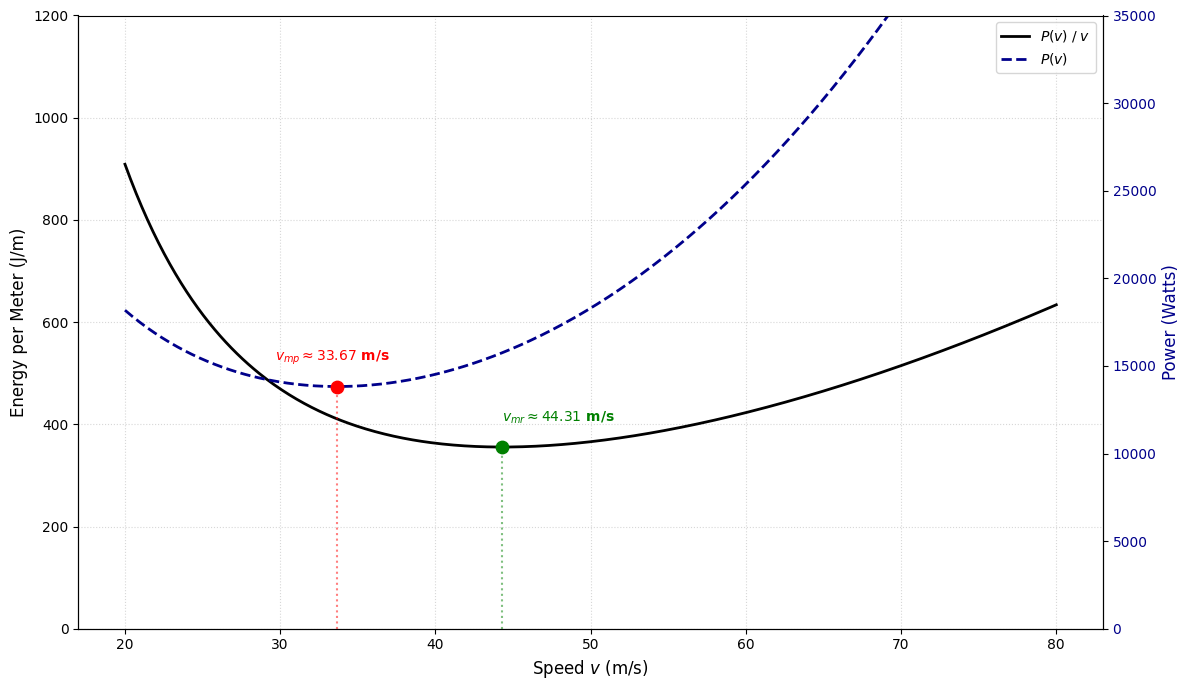
\includegraphics[width=100mm]{fig/output-2.png}
        \caption{Maximum-range speed versus minimum-power speed.}
        \label{fig:optimum-speed}
\end{figure}

 A natural modeling choice can be decomposing each flight leg into two parts with two separate speeds $v_1, v_2$, one for direct travel and one for loitering. The next result shows that this extended model offers no energy improvement, i.e., any decomposition of a flight leg into two parts traversed at distinct speeds consumes at least as much energy as a single uniform speed over the same total distance and total time as we state and prove in Theorem~(\ref{thm:single-speed}).
%
\begin{theorem}\label{thm:single-speed}
For any decomposition of a flight leg into two parts with positive lengths $d_1, d_2$ summing to $d$ and positive travel times $t_1, t_2$ summing to $t$, The energy function $E(d, t)$ defined in Equation~\eqref{eq:energy-dt} satisfies
\begin{equation}\label{eq:subadditive}
E(d, t) \;\le\;  E(d_1, t_1) + E(d_2, t_2).
\end{equation}
\end{theorem}
%
\begin{proof}
We express the energy function via the physical relation $v = d/t$ as $E(d, t) = t \cdot P(v)$, where the power function is given by $P(v) = c_0 + c_1 v^3 + c_2 / v$. 
Note that $P(v)$ is strictly convex for $v > 0$.

Let $v_1 = d_1/t_1$ and $v_2 = d_2/t_2$ be the speeds of the two parts. The average speed of the combined leg can be written as
\[
v \;=\; \frac{d_1 + d_2}{t_1 + t_2} \;=\; \left(\frac{t_1}{t_1 + t_2}\right) v_1 + \left(\frac{t_2}{t_1 + t_2}\right) v_2,
\]
which is a convex combination of $v_1$ and $v_2$. Applying the definition of convexity to $P(v)$ with $\lambda = t_1 / (t_1 + t_2) \in (0,1)$ gives
\[
P(v) \;\le\; \frac{t_1}{t_1 + t_2} P(v_1) + \frac{t_2}{t_1 + t_2} P(v_2).
\]
Multiplying both sides by the total travel time $t = t_1 + t_2$ yields
\[
t \, P(v) \;\le\; t_1 P(v_1) + t_2 P(v_2),
\]
which simplifies to the desired inequality $E(d, t) \le E(d_1, t_1) + E(d_2, t_2)$.
\end{proof}

\noindent

The UAV therefore optimally commits to a single speed $v_{ij}$ at the beginning of each leg $(i,j)$, justifying the single-speed assumption used throughout this paper, even when the leg carries enough time to satisfy a downstream time window, i.e., longer than the direct flight time $d_{ij}/v_{mr}$. From Equation~\eqref{eq:vmp}, the energy on a leg $(i,j)$ with fixed travel time $t_{ij}$ is minimized at $v_{ij} = v_{mp}$. Conversely, as long as the UAV is not pressured to fly faster or slower to meet a time window and the leg carries no loitering, we expect to see $v_{ij} = v_{mr}$, the speed that minimizes energy per unit distance.


%We model loitering implicitly in Section~\ref{sec:model} by allowing the length of a flight leg $L_{ij}$ between targets $i$ and $j$ to exceed the Euclidean distance $d_{ij}$, and the UAV maintains speed $v_{ij}$ along the leg.
% ============================================================
\subsection{MINLP formulation}\label{subsec:minlp}
% ============================================================
Building on the problem description of Section~\ref{subsec:problem} and the UAV energy consumption model of Section~\ref{subsec:uav}, we now formulate the UAV routing problem as a mixed-integer nonlinear program. The formulation contains four groups of decisions, namely binary indicators to select which targets to visit and which legs to fly, continuous arrival times at each visited target, continuous leg lengths, and continuous travel times, where the last two jointly encode the flight speed and any loitering.

To incorporate loitering into the formulation, we introduce the flight length variable $L_{ij} \ge d_{ij}$ for each leg $(i,j)$ and define travel time as
$
t_{ij} = L_{ij}/v_{ij}.
$
Since $L_{ij}$ may exceed $d_{ij}$, the travel time $t_{ij}$ naturally accounts for any additional loitering time. Substituting $v_{ij} = L_{ij}/t_{ij}$ into the energy function~\eqref{eq:energy} eliminates the speed variable and yields
\[
\sum_{\substack{i,j \in N \\ i \neq j}} \left( c_0\, t_{ij} + c_1 \frac{L_{ij}^3}{t_{ij}^2} + c_2 \frac{t_{ij}^2}{L_{ij}} \right) \le E_{\max},
\]
which, despite containing nonlinear terms, is amenable to a conic reformulation, derived in Section~\ref{subsec:misocp}. Based on the concepts provided in Section~\ref{subsec:problem}, the problem is first formulated as an MINLP model and then converted into its equivalent MISOCP model. The notation used in both models is summarized below.

\vspace{4mm}
\noindent\textbf{Sets and Indices}

\vspace{2mm}
\begin{tabular}{@{}l}
$N = \{0,1,\ldots,n\}$: set of all targets and the depot \\[6pt]

\end{tabular}

\vspace{4mm}

\noindent\textbf{Parameters}

\vspace{2mm}
\begin{tabular}{@{}l}
$d_{ij}$: Euclidean distance between targets $i$ and $j$ \\[6pt]
$T_{\max}$: mission time horizon \\[6pt]
$e_i$: earliest arrival time at target $i$ \\[6pt]
$\ell_i$: latest arrival time at target $i$ \\[6pt]
$I_{e_i}$: information available at time $e_i$ for target $i$ \\[6pt]
$\gamma_i$: information slope for target $i$ \\[6pt]
$v_{\min}, v_{\max}$: minimum and maximum UAV speeds \\[6pt]
$c_0, c_1, c_2$: energy consumption coefficients \\[6pt]
$E_{\max}$: energy budget \\[6pt]
$\gamma_0 = I_{e_0} = e_0 = 0$, \; $\ell_0 = T_{\max}$
\end{tabular}


\vspace{4mm}


\noindent\textbf{Decision Variables}

\vspace{2mm}
\begin{tabular}{@{}l}
$w_i =
\begin{cases}
1 & \text{if target $i$ is visited}, \quad i \in N\\
0 & \text{otherwise}
\end{cases}
$\\[16pt]

$x_{ij} =
\begin{cases}
1 & \text{if the UAV travels from target $i$ to $j$}, \quad i, j \in N,\; i \neq j\\
0 & \text{otherwise}
\end{cases}
$\\[14pt]
 $t_{ij}$: travel time from target $i$ to $j$, \quad $i, j \in N,\; i \neq j$ \\[6pt]
$a_i$: arrival time at target $i$, \quad $i \in N \setminus \{0\}$ \\[6pt]
$a_0$: arrival time back at the depot \\[6pt]
$L_{ij}$: flight length of leg $(i,j)$, \quad $i, j \in N,\; i \neq j$
\end{tabular}

\vspace{6mm}


\noindent\textbf{MINLP Formulation}
\begin{align}
    \max \quad & \sum_{i \in N} \bigl[ I_{e_i}\, w_i + \gamma_i (a_i - e_i\, w_i) \bigr] \label{minlp:obj} \\[6pt]
    \text{subject to} \notag \\[6pt]
& w_0 = 1 \label{minlp:depot}\\[6pt]
& \sum_{\substack{j \in N \\ j \neq i}} x_{ji} = \sum_{\substack{j \in N \\ j \neq i}} x_{ij} = w_i,
    && \forall\, i \in N \label{minlp:eulerian}\\
& e_i\, w_i \le a_i \le \ell_i\, w_i,
    && \forall\, i \in N \label{minlp:tw} \\[6pt]
& L_{ij} \ge d_{ij}\, x_{ij},
    && \forall\, i,j \in N,\; i \neq j \label{minlp:flight-length} \\[6pt]
& v_{\min}\, t_{ij} \le L_{ij} \le v_{\max}\, t_{ij},
    && \forall\, i,j \in N,\; i \neq j \label{minlp:distance-bound} \\[6pt]
& a_j \ge a_i + t_{ij} - \ell_i\, (1 - x_{ij}),
    && \substack{\forall\, i \in N \setminus \{0\}, \\ \forall\, j \in N,\; i \neq j} \label{minlp:timelink} \\[6pt]
& a_j \le a_i + t_{ij} + \ell_j\, (1 - x_{ij}),
    && \substack{\forall\, i \in N \setminus \{0\}, \\ \forall\, j \in N,\; i \neq j} \label{minlp:timelink2} \\[6pt]
& a_j \ge t_{0j},
    && \forall\, j \in N \setminus \{0\} \label{minlp:timelink-depot} \\[6pt]
& a_j \le t_{0j} + \ell_j\, (1 - x_{0j}),
    && \forall\, j \in N \setminus \{0\} \label{minlp:timelink-depot2} \\[6pt]
& t_{ij} \leq T_{\max}\, x_{ij},
    && \forall\, i,j \in N,\; i \neq j \label{minlp:time-bound} \\[6pt]
& \sum_{\substack{i,j \in N \\ i \neq j}} \left( c_0\, t_{ij} + c_1 \frac{L_{ij}^3}{t_{ij}^2} + c_2 \frac{t_{ij}^2}{L_{ij}} \right) \le E_{\max} \label{minlp:energy} \\
& w_i, x_{ij} \in \{0,1\}, \quad a_{i}, t_{ij} \geq 0 \label{minlp:domain}
\end{align}

The objective~\eqref{minlp:obj} maximizes total collected information based on arrival times at visited targets. Constraint~\eqref{minlp:depot} ensures the depot is always included. Flow conservation constraints~\eqref{minlp:eulerian} require that each visited target has exactly one incoming and one outgoing leg. Time window constraints~\eqref{minlp:tw} bound arrival times and force zero reward for unvisited targets (since $a_i = 0$ when $w_i = 0$). Flight length constraint~\eqref{minlp:flight-length} sets $L_{ij} \ge d_{ij}$ on travel legs, allowing loitering when $L_{ij} > d_{ij}$. Speed bounds~\eqref{minlp:distance-bound} link flight length and travel time. Time-precedence constraints~\eqref{minlp:timelink}--\eqref{minlp:timelink-depot2} synchronize arrival times along the route, while constraint~\eqref{minlp:time-bound} forces $t_{ij} = 0$ on inactive legs. The energy budget~\eqref{minlp:energy} limits total consumption, and~\eqref{minlp:domain} specifies variable domains.

Constraints~\eqref{minlp:timelink}--\eqref{minlp:timelink-depot2} also eliminate subtours since travel times are strictly positive on flight legs and arrival times increase monotonically along the route, preventing closed cycles. This monotonicity is relaxed only at the depot, which serves as the unique start and end point.

The time links are switched off on legs that are not flown by the constants $\ell_i$ and $\ell_j$ rather than by the horizon $T_{\max}$, and these are the tightest valid choices. Constraint~\eqref{minlp:time-bound} forces $t_{ij} = 0$ whenever $x_{ij} = 0$, and the window constraints~\eqref{minlp:tw} keep every arrival between zero and its window close, so $a_i - a_j \le \ell_i$ and $a_j - a_i \le \ell_j$ hold in every feasible solution and no schedule is cut off, while the depot-out lower link~\eqref{minlp:timelink-depot} needs no constant at all. Replacing the global horizon by these per-leg constants is the orienteering counterpart of the classical tightening of~\citep{desrochers1991improvements} for time-window formulations. It removes timing slack from the continuous relaxation without changing the integer feasible set.

The energy budget constraint~\eqref{minlp:energy} is the sole source of nonlinearity in the model; the next section reformulates it via rotated second-order cones to obtain a convex mixed-integer program solvable by standard MISOCP solvers.


% ============================================================
\subsection{MISOCP reformulation}\label{subsec:misocp}
% ============================================================

A \emph{second-order cone program} (SOCP) is a convex optimization problem of the form
\begin{equation}\label{eq:socp-standard}
\min_{x \in \mathbb{R}^{n}} \quad c^{\top} x \qquad \text{subject to} \qquad \lVert A_i\, x + b_i \rVert_{2} \;\le\; d_i^{\top}\, x + e_i, \quad i = 1, \dots, m,
\end{equation}
where each constraint requires the affine vector $A_i x + b_i$ to lie inside the second-order (Lorentz) cone of dimension matching its row count. Linear equalities and inequalities are special cases of~\eqref{eq:socp-standard}, recovered by taking $A_i = 0$, so any mixed linear–conic system fits the same framework~\cite{boyd2004convex}. When a subset of the variables is required to be integer, the problem becomes a \emph{mixed-integer second-order cone program} (MISOCP), which modern solvers (e.g., Gurobi, Mosek) handle by branch-and-bound with continuous SOCP relaxations at each node.


The energy constraint~\eqref{minlp:energy} contains nonlinear terms $L_{ij}^3/t_{ij}^2$ and $t_{ij}^2/L_{ij}$ that prevent direct solution as a mixed-integer linear or conic program. We reformulate these terms using auxiliary variables and rotated second-order cones.

Since $t_{ij}$ and $L_{ij}$ are forced to zero on inactive flight legs by constraints~\eqref{minlp:distance-bound} and~\eqref{minlp:time-bound}, the $x_{ij}$ multipliers can be omitted from the energy constraint without affecting optimality. We introduce auxiliary variables.
\begin{itemize}
    \item $z_{ij} \ge t_{ij}^2 / L_{ij}$, representable directly as a rotated second-order cone;
    \item $s_{ij} \ge L_{ij}^2 / t_{ij}$, an intermediate variable needed to decompose the cubic term;
    \item $y_{ij} \ge s_{ij}^2 / L_{ij} = L_{ij}^3 / t_{ij}^2$, completing the decomposition.
\end{itemize}

\noindent The MISOCP formulation replaces~\eqref{minlp:energy} with the following constraints.

\begin{align}
\max \quad & \sum_{i \in N} \bigl[ I_{e_i}\, w_i + \gamma_i (a_i - e_i\, w_i) \bigr] \label{misocp:obj} \\[6pt]
\text{subject to} & \quad \eqref{minlp:depot}\text{--}\eqref{minlp:time-bound},\; \eqref{minlp:domain}, \notag \\[6pt]
& \sum_{\substack{i,j \in N  \\ i \neq j}} \left( c_0\, t_{ij} + c_1\, y_{ij} + c_2\, z_{ij} \right) \le E_{\max} \label{misocp:energy} \\[6pt]
& \left\lVert
    \begin{pmatrix}
        t_{ij} \\[2pt]
        \frac{z_{ij}-L_{ij}}{2}
    \end{pmatrix}
 \right\rVert_2
 \le \frac{z_{ij}+L_{ij}}{2}, && \forall\, i,j \in N,\; i \neq j \label{misocp:cone-z} \\[6pt]
& \left\lVert
    \begin{pmatrix}
        L_{ij} \\[2pt]
        \frac{t_{ij}-s_{ij}}{2}
    \end{pmatrix}
 \right\rVert_2
 \le \frac{t_{ij}+s_{ij}}{2}, && \forall\, i,j \in N,\; i \neq j \label{misocp:cone-s} \\[6pt]
& \left\lVert
    \begin{pmatrix}
        s_{ij} \\[2pt]
        \frac{L_{ij}-y_{ij}}{2}
    \end{pmatrix}
 \right\rVert_2
 \le \frac{L_{ij}+y_{ij}}{2}, && \forall\, i,j \in N,\; i \neq j \label{misocp:cone-y} \\[6pt]
& y_{ij} \leq v_{\max}^3\, t_{ij},
    && \forall\, i,j \in N,\; i \neq j \label{misocp:y-bound} \\[6pt]
& z_{ij} \leq t_{ij} / v_{\min},
    && \forall\, i,j \in N,\; i \neq j \label{misocp:z-bound} \\[6pt]
&  s_{ij},\, y_{ij},\, z_{ij} \ge 0 && \forall\, i,j \in N,\; i \neq j \notag
\end{align}

Each cone constraint encodes a rotated second-order cone of the form $u^2 \le ab$ (with $a, b \ge 0$).
\begin{itemize}
    \item Constraint~\eqref{misocp:cone-z} gives $t_{ij}^2 \le z_{ij} \cdot L_{ij}$, so $z_{ij} \ge t_{ij}^2 / L_{ij}$.
    \item Constraint~\eqref{misocp:cone-s} gives $L_{ij}^2 \le t_{ij} \cdot s_{ij}$, so $s_{ij} \ge L_{ij}^2 / t_{ij}$.
    \item Constraint~\eqref{misocp:cone-y} gives $s_{ij}^2 \le L_{ij} \cdot y_{ij}$, so $y_{ij} \ge s_{ij}^2 / L_{ij} \ge L_{ij}^3 / t_{ij}^2$.
\end{itemize}
Bounds~\eqref{misocp:y-bound} and~\eqref{misocp:z-bound} tighten the relaxation and ensure that auxiliary variables collapse to zero on inactive legs, improving numerical stability and branch-and-bound performance. 
The information-maximizing objective~\eqref{misocp:obj} is indifferent between two solutions that visit the same target set with the same arrival times but differ in the speeds (equivalently, flight lengths $L_{ij}$) assigned to legs along which no time window or downstream arrival is binding. To remove this degeneracy and select a unique energy-optimal speed on every leg, the natural reference is a lexicographic objective that maximizes total information first and, among all information-optimal solutions, minimizes total energy. Two implementations realize this lexicographic order.
\begin{enumerate}
    \item[(i)] \emph{Two-stage solve.} First solve~\eqref{misocp:obj} to obtain the maximum information value~$f^\star$, then re-solve with the constraint $\sum_i [I_{e_i} w_i + \gamma_i (a_i - e_i w_i)] \ge f^\star$ and a minimum-energy objective. This is exact (the two stages cannot trade information for energy) but requires two MISOCP solves per instance, the second of which carries an additional equality-like constraint that tightens the LP relaxation only marginally and roughly doubles the solver time.
    \item[(ii)] \emph{Penalized objective.} Augment the objective with an energy term scaled small enough that no information-equivalent trade is profitable.
    \begin{equation}\label{eq:tiebreaker}
    \max \quad \sum_{i \in N} \bigl[ I_{e_i}\, w_i + \gamma_i (a_i - e_i\, w_i) \bigr] \;-\; \varepsilon\, \frac{1}{E_{\max}} \sum_{\substack{i, j \in N \\ i \neq j}} \bigl( c_0\, t_{ij} + c_1\, y_{ij} + c_2\, z_{ij} \bigr),
    \end{equation}
    where $\varepsilon$ is a small positive parameter chosen so that the resulting change in the maximum information value is negligible. The penalty's magnitude is bounded by $\varepsilon$ since the energy ratio is at most one, which is orders of magnitude below any per-target reward. Among information-equivalent solutions, the penalty selects the one with the smallest total energy.
\end{enumerate}
We adopt option~(ii) throughout this paper. It introduces no additional constraints and requires a single MISOCP solve per instance, which is essential for the matheuristic of Section~\ref{sec:heuristic}, where the SOCP subproblem is solved thousands of times to evaluate candidate routes. This has two practical consequences observed in our experiments. (i)~The reported total energy may fall below $100\%$ of $E_{\max}$ when the information optimum does not exhaust the budget. (ii)~On flight legs with no binding time window (e.g., the return leg to the depot), the solver flies at the maximum-range speed $v_{mr}$ from Equation~\eqref{eq:vmr} rather than at an arbitrary feasible speed, since $v_{mr}$ minimizes energy per meter. We apply the same tie-breaker to the fixed-tour SOCP subproblem of Section~\ref{subsec:socp}.

\section{A Matheuristic Based on Iterated Local Search}\label{sec:heuristic}

The MISOCP formulation of Section~\ref{subsec:misocp} simultaneously determines four decisions, namely the subset of targets to visit, the visiting order, and the travel distance and travel time on every flight leg. Moreover, each flight leg requires three auxiliary conic constraints~\eqref{misocp:cone-z}--\eqref{misocp:cone-y}, causing the model size to grow quadratically with $|N|$. Practical reconnaissance missions may involve hundreds of candidate targets, far beyond what a branch-and-bound search over this conic model can be expected to certify, which motivates a scalable solution approach.

Our solution approach decomposes these decisions into two interconnected subproblems. The first determines the subset of targets to visit together with their visiting order, thereby defining a closed tour. The second optimizes the travel distance and travel time on each flight leg for a fixed tour. Since this subproblem is convex, it can be solved to optimality by the SOCP model of Section~\ref{subsec:socp}.

Building on this decomposition, we develop a matheuristic in the form of an Iterated Local Search (ILS). The outer search explores the combinatorial space through neighborhood moves, while the inner SOCP computes the optimal continuous decisions for every candidate tour. The search is initialized from one of four construction heuristics, repeatedly improved by local search, and diversified through a shake step whenever the local search has exhausted the neighborhood of its route. Every candidate route costs one solve of the subproblem, so the design question is which routes deserve that solve. Section~\ref{subsec:proposal} answers it with exact feasibility tests and candidate weights that need no subproblem, and Section~\ref{subsec:ils} with a shake step that is applied systematically rather than at random.

% ============================================================
\subsection{Fixed-tour SOCP subproblem}\label{subsec:socp}
% ===========================================================

We first make precise what the combinatorial side of the decomposition hands
to the continuous side. A \emph{route} is a sequence $R = (0, r_1, r_2, \ldots,
r_k, 0)$ that starts and ends at the depot and schedules $k \ge 1$ distinct targets
$r_1, \ldots, r_k \in N \setminus \{0\}$, each exactly once. A route fixes the
target selection and visiting order while leaving the associated continuous decisions
unspecified. Every feasible solution of the MINLP in Section~\ref{subsec:minlp}
induces exactly one such route, since the time-precedence
constraints~\eqref{minlp:timelink}--\eqref{minlp:timelink-depot2}
exclude subtours. Thus, the MINLP can equivalently be viewed as selecting a route
together with its associated continuous decisions. Let $N_R = \{0, r_1, \ldots, r_k\}$
denote the scheduled targets of a route $R$, the depot included, and $A_R = \{(0,r_1), (r_1,r_2), \ldots, (r_{k-1},r_k),
(r_k,0)\}$ its flight legs. We use the words route and tour interchangeably. Along a route the depot is left at time zero and $a_0$ denotes the return time, which the depot window $[0, T_{\max}]$ of Section~\ref{subsec:problem} bounds.

For a given route $R$, the remaining subproblem optimizes the travel times and flight lengths, equivalently the corresponding speeds, along the route to maximize information collection subject to the energy budget. Since the visited targets and the flown legs are known, the binary variables of the MINLP formulation of Section~\ref{subsec:minlp} are fixed, with $w_i = 1$ on $N_R$, $x_{ij} = 1$ on $A_R$, and both zero elsewhere. Consequently, the objective no longer contains the target-selection variables, the time windows become simple bounds, and the time-precedence constraints simplify to equalities. The resulting formulation is the following continuous nonlinear program (NLP).

\vspace{4mm}
\noindent\textbf{NLP Formulation}
\begin{align}
\max \quad
& \sum_{i \in N_R \setminus \{0\}} \bigl(\gamma_i\, a_i - \gamma_i\, e_i + I_{e_i} \bigr) \label{nlp:obj} \\[6pt]
\text{subject to} \notag \\[6pt]
& \sum_{(i,j) \in A_R} \left( c_0\, t_{ij} + c_1 \frac{L_{ij}^3}{t_{ij}^2} + c_2 \frac{t_{ij}^2}{L_{ij}} \right) \le E_{\max} \label{nlp:energy} \\[6pt]
& L_{ij} \ge d_{ij},
    && \forall\, (i,j) \in A_R \label{nlp:path-length} \\[6pt]
& v_{\min}\, t_{ij} \le L_{ij} \le v_{\max}\, t_{ij},
    && \forall\, (i,j) \in A_R \label{nlp:speed-bound} \\[6pt]
& e_i \le a_i \le \ell_i,
    && \forall\, i \in N_R \label{nlp:timewindow} \\[6pt]
& a_j = a_i + t_{ij},
    && \forall\, (i,j) \in A_R \setminus \{(0,r_1)\} \label{nlp:timelink} \\[6pt]
& a_{r_1} = t_{0,r_1} \label{nlp:timelink-depot} \\[6pt]
& t_{ij},\, L_{ij} \ge 0,
    && \forall\, (i,j) \in A_R. \label{nlp:domain}
\end{align}

Because the tour sequence is fixed, the time-precedence inequalities~\eqref{minlp:timelink}--\eqref{minlp:timelink-depot2} reduce to the equalities~\eqref{nlp:timelink}--\eqref{nlp:timelink-depot}. Since $d_{ij}>0$ for all flight legs in $A_R$, constraint~\eqref{nlp:speed-bound} implies $t_{ij}>0$, which in turn guarantees $a_j>a_i$ along the tour through~\eqref{nlp:timelink}. Applying the same conic reformulation and the same energy tie-breaker with the same small positive $\varepsilon$ as in Section~\ref{subsec:misocp}, we obtain the following SOCP formulation for a given route $R$.

\vspace{4mm}
\noindent\textbf{SOCP Formulation}
\begin{align}
\max \quad
& \sum_{i \in N_R \setminus \{0\}} \bigl(\gamma_i\, a_i - \gamma_i\, e_i + I_{e_i} \bigr)
\;-\; \varepsilon\, \frac{1}{E_{\max}}
\sum_{(i,j) \in A_R}
\bigl( c_0\, t_{ij} + c_1\, y_{ij} + c_2\, z_{ij} \bigr)
\label{socp:obj} \\[6pt]
\text{subject to} \quad
& \eqref{nlp:path-length}\text{--}\eqref{nlp:domain}, \notag \\[6pt]
& \sum_{(i,j) \in A_R}
\left( c_0\, t_{ij} + c_1\, y_{ij} + c_2\, z_{ij} \right)
\le E_{\max} \label{socp:energy} \\[6pt]
& \left\lVert
\begin{pmatrix}
t_{ij} \\[2pt]
\frac{z_{ij}-L_{ij}}{2}
\end{pmatrix}
\right\rVert_2
\le \frac{z_{ij}+L_{ij}}{2},
&& \forall\, (i,j) \in A_R \label{socp:cone-z} \\[6pt]
& \left\lVert
\begin{pmatrix}
L_{ij} \\[2pt]
\frac{t_{ij}-s_{ij}}{2}
\end{pmatrix}
\right\rVert_2
\le \frac{t_{ij}+s_{ij}}{2},
&& \forall\, (i,j) \in A_R \label{socp:cone-s} \\[6pt]
& \left\lVert
\begin{pmatrix}
s_{ij} \\[2pt]
\frac{L_{ij}-y_{ij}}{2}
\end{pmatrix}
\right\rVert_2
\le \frac{L_{ij}+y_{ij}}{2},
&& \forall\, (i,j) \in A_R \label{socp:cone-y} \\[6pt]
& s_{ij},\, y_{ij},\, z_{ij} \ge 0,
&& \forall\, (i,j) \in A_R. \notag
\end{align}

The resulting SOCP is a continuous convex program that can be solved efficiently by modern solvers. It is used to evaluate every route generated by the local search. At each step, the ILS proposes a new route by modifying the target sequence, and the SOCP optimizes the associated continuous decisions and returns the resulting objective value. Thus, the ILS does not need to search over the continuous decision space.

We call a route \emph{SOCP-feasible} if this subproblem admits a feasible solution. Whether a route is SOCP-feasible depends on its time windows, the mission horizon, and the energy budget, so feasibility is determined by the continuous subproblem rather than by the route structure alone. For simplicity, for an SOCP-feasible route $R$ we write $f(R)$ for the optimal value of~\eqref{socp:obj}, and $E_R$ and $T_R$ for the energy term of the budget constraint~\eqref{socp:energy} and the return time $a_0$ of the solution the subproblem returns. The value $f(R)$ is uniquely determined as an optimal value; the energy $E_R$ is pinned by the tie-breaker among information-equivalent schedules, and the return time can differ between alternative optimal schedules, which is why both are tied to the returned solution and read within the solver's tolerance. These three route quantities are what the construction heuristics and the local search compare. The decision variables themselves never leave the subproblem.

\paragraph{Units.}
The subproblem is passed to the solver in the nondimensional units of Section~\ref{subsec:mapping}: lengths are divided by the range $E_{\max}/\bar{e}$ that the budget at $\eta = 1$ buys at the maximum-range speed, with $\bar{e} = P(v_{mr})/v_{mr}$ the minimum energy per meter, times by that range over $v_{mr}$, speeds by $v_{mr}$ and energy by the budget. In these units the two propulsion coefficients both become $1/2$, every variable of the cone model is of order one, and the objective is unchanged. In physical units the coefficients of the same model span more than seven decades, the barrier method needs its most conservative numerical settings, and presolve declares feasible routes infeasible; in the scaled units the default settings, with presolve disabled and the homogeneous barrier, return the same feasibility verdicts and the same values within the solver tolerance in a fraction of the barrier iterations, as Section~\ref{subsec:parameter-analysis} reports. Since the subproblem is solved for every candidate route, its solve time is the unit in which the cost of the search is measured, and everything that follows is designed to spend it only where it can pay.

% ============================================================
\subsection{Construction heuristics}\label{subsec:initial}
% ============================================================

The iterated local search of Section~\ref{subsec:ils} starts from an initial solution built by a construction heuristic. We keep the route notation $R = (0, r_1, \ldots, r_k, 0)$ of Section~\ref{subsec:socp}, with the scheduled targets $N_R$ written by position, and write $N' = N \setminus N_R$ for the set of unscheduled targets. Inserting an unscheduled target $u \in N'$ at position $p \in \{1, \ldots, k+1\}$ of $R$ yields the route
\[
R \oplus \langle u, p \rangle \;=\; (0, r_1, \ldots, r_{p-1}, u, r_p, \ldots, r_k, 0),
\]
and the insertion $\langle u, p \rangle$ is \emph{SOCP-feasible} in the sense of Section~\ref{subsec:socp} if this route admits travel times and flight lengths that satisfy every time window, the mission horizon, and the energy budget.

All four construction heuristics start from the depot alone, $R_0 = (0)$, and repeatedly append a target at the last position, $p = k+1$, so that the first append gives $k = 1$ and every intermediate route is SOCP-feasible. Feasibility is verified in R1 to R4 by solving the SOCP subproblem on the candidate route, and $N'$ is updated after every append. The heuristics differ only in the rule that selects the target to append.

\begin{enumerate}[label=\textbf{R\arabic*}., leftmargin=2em]
\item \textbf{Earliest opening.}
The targets $u \in N'$ are sorted by the opening time $e_u$ of their time windows $W_u$ and the first target whose insertion is SOCP-feasible is appended. The procedure stops once $k = 4$.

\item \textbf{Random then earliest opening.}
The first target is selected uniformly at random among the targets in $N'$ whose insertion is SOCP-feasible. The remaining targets are appended by the rule of R1 until $k = 4$.

\item \textbf{Random.}
Targets are drawn uniformly at random from $N'$ and appended whenever the insertion is SOCP-feasible, until $k = 4$.

\item \textbf{Greedy.}
Among the SOCP-feasible extensions, the target with the highest collected information per unit of capacity is appended,
\begin{equation}\label{eq:r4-ratio}
u^{*} \;=\; \arg\max_{u \in N'} \; \frac{f(R \oplus \langle u, k+1 \rangle)}{\mathrm{cap}(R \oplus \langle u, k+1 \rangle)},
\qquad
\mathrm{cap}(R) \;=\; \max\!\left\{ \frac{T_R}{T_{\max}},\; \frac{E_R}{E_{\max}} \right\},
\end{equation}
where $f(R)$, $T_R$ and $E_R$ are the route quantities of Section~\ref{subsec:socp}. The capacity $\mathrm{cap}(R)$ is the larger of the two normalized resource utilizations of the route, so it measures the resource that binds first, and the quotient measures the information the route collects per unit of that resource. The procedure stops when no SOCP-feasible insertion remains.
\end{enumerate}

The quotient in~\eqref{eq:r4-ratio} plays the role of the insertion ratio of \citep{vansteenwegen2009iterated}, which divides the square of a visit's score by the time its insertion consumes. Two differences follow from our problem. A change of the route changes the arrival times of every target, since the subproblem reschedules the whole route, so the quotient is a property of the route rather than of one visit. And two resources rather than one are consumed. Dividing by either one alone would prefer a target that is cheap in that resource while exhausting the other, whereas normalizing each by its own limit makes the two comparable, so the maximum in~\eqref{eq:r4-ratio} charges every candidate for the resource it actually depletes. Heuristics R1 to R3 stop at $k = 4$, which leaves the route length to the local search rather than to the starting rule. R4 is the greedy construction heuristic and the default starting point of the search. Section~\ref{subsec:initial-selection} compares the four starting points.

% ============================================================
\subsection{Local search}\label{subsec:proposal}\label{subsec:operators}
% ============================================================

The local search modifies the current route $R = (0, r_1, \ldots, r_k, 0)$ with four operators.
\begin{enumerate}[noitemsep, topsep=4pt, leftmargin=2em]
    \item \textbf{Insert} inserts one unscheduled target $u \in N'$ at a position $p \in \{1, \ldots, k+1\}$ of the route, between $r_{p-1}$ and $r_p$.
    \item \textbf{Replace} replaces the scheduled target $r_p$ at position $p \in \{1, \ldots, k\}$ by an unscheduled target $u \in N'$. The number of scheduled targets is unchanged.
    \item \textbf{Swap} exchanges two scheduled targets $r_p$ and $r_q$, $1 \le p < q \le k$.
    \item \textbf{2-opt} reverses the sequence of scheduled targets between two positions $p$ and $q$, $1 \le p < q \le k$.
\end{enumerate}
Insert and Replace change the set of scheduled targets, while Swap and 2-opt change only their order. A move is denoted by $m$ and the route it produces by $R \circ m$, so that $R \circ \langle u, p \rangle = R \oplus \langle u, p \rangle$ for an Insert move.

Each iteration of the local search applies one operator to the current route. The operator is selected uniformly at random among those that apply to the route, where Swap requires at least two and 2-opt at least three scheduled targets, the set of feasible moves of that operator is determined, one move is drawn from it, and the resulting route is evaluated by the SOCP subproblem of Section~\ref{subsec:socp} and submitted to the acceptance criterion of Section~\ref{subsec:ils}. This differs from the iterated local searches of \citep{gunawan2015iterated, gunawan2017well}, which apply the four operators in a fixed sequence, each until no further improvement is found, and from the iterated local search of \citep{vansteenwegen2009iterated}, which applies Insert only. A fixed sequence is well suited to an evaluation in constant time, whereas every evaluation in our setting requires solving the SOCP subproblem, so the search is organized as a sequence of single moves and the operators are drawn at random.

\paragraph{Leg feasibility.}
A condition that depends on the instance alone restricts the candidates for a slot before any route is examined. On a flown leg $(i,j)$ the length constraint~\eqref{nlp:path-length} and the speed bound~\eqref{nlp:speed-bound} give $t_{ij} \ge d_{ij}/v_{\max}$, the time link~\eqref{nlp:timelink} gives $a_j = a_i + t_{ij}$, and the time windows~\eqref{nlp:timewindow} give $a_i \ge e_i$ and $a_j \le \ell_j$, so every leg of a feasible route satisfies
\begin{equation}\label{eq:leg-cond}
    e_i \;+\; d_{ij} / v_{\max} \;\le\; \ell_j .
\end{equation}
Loitering leaves the travel time unbounded above, so $v_{\min}$ yields no such condition. We compute once, in $O(|N|^2)$ time, the sets
\begin{equation}\label{eq:fb-sets}
    F_i \;=\; \{\, u \in N : e_i + d_{iu}/v_{\max} \le \ell_u \,\}
    \qquad \text{and} \qquad
    B_i \;=\; \{\, u \in N : e_u + d_{ui}/v_{\max} \le \ell_i \,\}
\end{equation}
of the targets that may directly follow $i$ and that may directly precede $i$, with $e_0 = 0$ and $\ell_0 = T_{\max}$ at the depot. They are the row and the column of one table, since $u \in B_i$ holds exactly when $i \in F_u$. Condition~\eqref{eq:leg-cond} is the time window elimination of flight legs of \citep{desrochers1991improvements}, and it implies the weaker compatibility condition $\ell_u > e_i$ on which \citep{vansteenwegen2009iterated} and \citep{gunawan2015iterated} rely. By the triangle inequality on the leg distances, $a_{r_j} \ge a_{r_i} + d_{r_i, r_j}/v_{\max}$ for any two positions $i < j$ of a route, so the condition holds for every ordered pair and not only for consecutive ones, that is $r_j \in F_{r_i}$ whenever $i < j$. Two targets that fail it in both directions never share a route.

Condition~\eqref{eq:leg-cond} bounds one leg at a time and starts it at the window opening of its first target. Chained along the current route it accumulates the travel times of all earlier legs and yields the arrival bounds
\begin{equation}\label{eq:leg-chain}
\begin{aligned}
    a^{\min}_{r_0} &= 0, &\qquad
    a^{\min}_{r_q} &= \max\!\bigl( e_{r_q},\; a^{\min}_{r_{q-1}} + d_{r_{q-1}, r_q} / v_{\max} \bigr), &\quad q &= 1, \ldots, k+1, \\
    a^{\max}_{r_{k+1}} &= T_{\max}, &\qquad
    a^{\max}_{r_q} &= \min\!\bigl( \ell_{r_q},\; a^{\max}_{r_{q+1}} - d_{r_q, r_{q+1}} / v_{\max} \bigr), &\quad q &= k, \ldots, 1,
\end{aligned}
\end{equation}
both computed in $O(k)$ time from the route alone, with $r_{k+1} = 0$ the return to the depot. The forward bound is the earliest arrival that the route prefix permits, since no leg is flown faster than $v_{\max}$ along the straight line and waiting only adds time, and the backward bound is the latest arrival that keeps every later window and the return to the depot reachable. Placing a target $u$ between two consecutive route members $i$ and $j$ satisfies every time window if and only if
\begin{equation}\label{eq:slot-test}
    \max\!\bigl( e_u,\; a^{\min}_i + d_{iu} / v_{\max} \bigr)
    \;\le\;
    \min\!\bigl( \ell_u,\; a^{\max}_j - d_{uj} / v_{\max} \bigr),
\end{equation}
because any travel time longer than $d / v_{\max}$ is realizable by flying slower or by loitering, so the test is exact for the variable speed model and leaves only the energy budget to the subproblem.

Intersecting the two bounds with the window of the target gives the \emph{realized window}
\begin{equation}\label{eq:realized-window}
    \bar{W}_{r_q} \;=\; W_{r_q} \cap \bigl[\, a^{\min}_{r_q},\; a^{\max}_{r_q} \,\bigr] \;=\; \bigl[\, a^{\min}_{r_q},\; a^{\max}_{r_q} \,\bigr] ,
\end{equation}
the two forms agreeing because the recursion~\eqref{eq:leg-chain} intersects with the window at every step. It is the part of the window that the rest of the route leaves available: every arrival time in it is met by some schedule that respects all windows, and no time outside it is. The route satisfies every time window if and only if $\bar{W}_{r_q} \neq \emptyset$, that is $a^{\min}_{r_q} \le a^{\max}_{r_q}$, at every position $q$, and a move whose route has an empty realized window anywhere is discarded before any subproblem is solved. Test~\eqref{eq:slot-test} is this condition written for the one position that a slot insertion adds.

The one-leg condition needs no separate check. Since $a^{\min}_i \ge e_i$ and $a^{\max}_j \le \ell_j$, the test~\eqref{eq:slot-test} gives $e_i + d_{iu}/v_{\max} \le \ell_u$ and $e_u + d_{uj}/v_{\max} \le \ell_j$, that is $u \in F_i \cap B_j$, and~\eqref{eq:leg-cond} is~\eqref{eq:slot-test} with the two arrival bounds replaced by the window ends. The sets are the building block from which~\eqref{eq:leg-chain} is chained, and in the implementation they are intersected to enumerate the candidates of a slot rather than scanning every unscheduled target. Insert $\langle u, p \rangle$ is tested by~\eqref{eq:slot-test} with $i = r_{p-1}$ and $j = r_p$, and Replace $\langle u, p \rangle$ with $i = r_{p-1}$ and $j = r_{p+1}$, both in $O(1)$ time, since the prefix before the slot and the suffix after it are unchanged and their bounds are those of $R$.

\paragraph{Reorderings in constant time.}
Swap and 2-opt reorder several targets at once, and recomputing the bounds~\eqref{eq:leg-chain} of every reordered route would cost $O(k)$ per position pair and $O(k^3)$ per route. The test is decided in $O(1)$ per pair instead by summarizing the reordered part of the route. For a segment $\sigma = (s_1, \ldots, s_m)$ of targets flown in this order, let the arrival at $s_1$ be $a \ge e_{s_1}$. The earliest arrival at $s_m$ that the segment permits is then $\max(a + D_\sigma, W_\sigma)$, and every window of the segment is met if and only if $a \le L_\sigma$, where $D_\sigma$ is the travel time of the segment at $v_{\max}$, $W_\sigma$ the earliest arrival at $s_m$ forced by the windows inside the segment, and $L_\sigma$ the latest entry that keeps those windows reachable. A single target $s$ has $D = 0$, $W = e_s$ and $L = \ell_s$, and the three numbers of a longer segment follow from those of a shorter one in $O(1)$ time. Placing a target $x$ in front of a segment whose first target is $y$, with $\tau = d_{xy}/v_{\max}$, gives
\begin{equation}\label{eq:seg-prepend}
    D' = \tau + D, \qquad W' = \max(e_y + D,\; W), \qquad
    L' = \begin{cases} \min(\ell_x,\; L - \tau) & \text{if } e_y \le L, \\ -\infty & \text{otherwise,} \end{cases}
\end{equation}
and appending a target $z$ after a segment whose last target is $w$, with $\tau = d_{wz}/v_{\max}$, gives
\begin{equation}\label{eq:seg-append}
    D' = D + \tau, \qquad W' = \max(W + \tau,\; e_z), \qquad
    L' = \begin{cases} \min(L,\; \ell_z - D - \tau) & \text{if } W + \tau \le \ell_z, \\ -\infty & \text{otherwise.} \end{cases}
\end{equation}
Both follow from the recursion~\eqref{eq:leg-chain} written for the segment, and $L' = -\infty$ records that some window of the segment is missed however early it is entered. This is the concatenation of time-window segments of \citep{savelsbergh1992vehicle}, in the form that allows waiting, which here is loitering. The 2-opt move $\langle p, q \rangle$ flies the prefix $(0, \ldots, r_{p-1})$, the reversed segment $(r_q, r_{q-1}, \ldots, r_p)$ and the suffix $(r_{q+1}, \ldots, 0)$; for a fixed $p$ the reversed segment of $q + 1$ is that of $q$ with $r_{q+1}$ placed in front, so~\eqref{eq:seg-prepend} yields its summary as $q$ advances. The Swap move $\langle p, q \rangle$ flies the prefix, $r_q$, the interior $(r_{p+1}, \ldots, r_{q-1})$, $r_p$ and the suffix; for a fixed $p$ the interior of $q + 1$ is that of $q$ with $r_q$ appended, so~\eqref{eq:seg-append} applies. In both cases the reordered route satisfies every time window if and only if the arrival at the first reordered target, $\max(e, a^{\min}_{r_{p-1}} + d/v_{\max})$, does not exceed the summary's $L$, and the earliest arrival at its last reordered target, read from the summary and carried over the connecting leg, does not exceed $a^{\max}_{r_{q+1}}$ of the unchanged suffix. The arrival bounds of $R$ serve every pair, so the Swap and 2-opt sets are built in $O(k^2)$ time, and every position pair that passes enters the set, whether the reordering shortens the route or lengthens it. On the longest routes the construction of these sets, and not the subproblem, was the dominant cost of an iteration; Section~\ref{subsec:parameter-analysis} quantifies the difference.

Swap and 2-opt interact with the time windows in a way that Insert and Replace do not. On instances whose time windows fix the visiting order, the reversed condition fails for most pairs and both operators are rejected in most iterations. Since this depends on the instance and not on the operators, both are kept in the local search, and Section~\ref{subsec:solomon} quantifies how often they can be applied on the benchmark instances.

\paragraph{Feasible moves.}
Since solving the SOCP subproblem is the most time-consuming step of an iteration, the local search determines the set $\mathcal{M}_o(R)$ of moves of an operator $o$ that pass the following two conditions before any subproblem is solved, and draws the move to evaluate from that set. Neither requires the subproblem.
\begin{enumerate}[noitemsep, topsep=4pt, leftmargin=2em]
    \item \textbf{Time window feasibility.} The route produced by the move passes the test~\eqref{eq:slot-test}, or for a reordering the concatenation test of~\eqref{eq:seg-prepend}--\eqref{eq:seg-append}.
    \item \textbf{Minimum energy of the route.} A leg consumes at least its length times $E(v_{mr}, 1)$, the energy per meter of~\eqref{eq:energy} at the maximum-range speed, but the time windows may force it to be flown at another speed and so to cost more. Read the schedule in cumulative distance: the cumulative arrival time must stay inside the time window $W_{r_q} = [e_{r_q}, \ell_{r_q}]$ at every target $r_q$ and inside $[0, T_{\max}]$ at the depot return. A leg of length $d$ flown in time $t$ has slope $s = t/d$ in that plane, so it is flown at speed $1/s$ and costs $d\,\psi(s)$ with
    \begin{equation}\label{eq:psi}
        \psi(s) = s\, P\!\bigl(\max(v_{mp},\, 1/s)\bigr),
    \end{equation}
    where $P$ is the power function of~\eqref{eq:power-full} and the $\max$ is loitering: given more time than $d/v_{mp}$ the drone holds the minimum-power speed $v_{mp}$ of~\eqref{eq:vmp} and flies the surplus, rather than fly slower and burn more. So $\psi(s) = E(1/s,\, 1)$ wherever $1/s \ge v_{mp}$, and minimizing it over $s$ is minimizing $P(v)/v$ over $v$, which by~\eqref{eq:vmr} is least at $v_{mr}$. The function is convex and minimal at the slope $s = 1/v_{mr}$. The minimum energy of the route over all schedules inside the windows is therefore attained by the tightest schedule the windows admit: piecewise linear, of constant slope between the points where it meets a window end, at the preferred slope $1/v_{mr}$ wherever the windows leave room. It is computed in $O(k)$ and the move is discarded when it exceeds $E_{\max}$. Where that schedule asks for a slope below $1/v_{\max}$ the speed it needs is unavailable, and the subproblem decides instead. The cheaper necessary condition that the route length times $\bar{e} = P(v_{mr})/v_{mr}$ stays within $E_{\max}$ is applied to every candidate while the set is built, and the exact test to the move that is drawn.
\end{enumerate}
A Replace move is treated as a removal followed by an insertion. Removing the scheduled target $r_p$ leaves the shorter route $R \ominus r_p$, and the Replace set is the union over the $k$ removals of the insertion set of $R \ominus r_p$, each one built and drawn as the Insert set of that route and weighted against $R$ itself, so that the estimate of the displaced target is charged to the move. Nothing in the construction refers to the reward the displaced target earns, so a replacement that loses information at the slot is not excluded: it may still raise the objective through the rescheduling of the rest of the route, and the acceptance criterion of Section~\ref{subsec:ils} is what refuses it if it does not.

Both conditions are exact, so the subproblem decides only whether a speed schedule within $[v_{\min}, v_{\max}]$ attains the minimum energy that this schedule certifies. With the bounds~\eqref{eq:leg-chain} at hand a slot is tested in $O(1)$ time, so the Insert and Replace sets are built in $O(k\,|N'|)$ time and the Swap and 2-opt sets in $O(k^2)$ time. Weighting a move requires the information estimate of the route it produces, whose cost is discussed next.

Two consequences follow from building a set once per route and removing every move that is drawn from it. An iteration whose operator has an empty set makes no move, and a route whose four sets are all empty admits no move at all, so the search leaves such a route only by the shake step of Section~\ref{subsec:ils}. Since every draw removes a move, every route reaches that state after finitely many draws.

\paragraph{Weight of a move.}
A move is weighted by the information it gains per unit of distance it adds, both of which are available without solving the subproblem. The move changes the route length by $\Delta d_m$, with the loitering of $R$ unchanged. For the insertion $\langle u, p \rangle$ this is the detour
\begin{equation}\label{eq:detour}
    \Delta d_{\langle u, p \rangle} \;=\; d_{r_{p-1}, u} + d_{u, r_p} - d_{r_{p-1}, r_p} \;\ge\; 0 ,
\end{equation}
nonnegative by the triangle inequality, and for the Replace move that puts $v$ in the place of $r_p$ it is the detour of $v$ into the gap the removal leaves,
\begin{equation}\label{eq:replace-weight}
    \Delta d_m \;=\; d_{r_{p-1}, v} + d_{v, r_{p+1}} - d_{r_{p-1}, r_{p+1}} \;\ge\; 0 .
\end{equation}
A reordering changes no member of the route, and its $\Delta d_m$ may have either sign. The added length is flown at the maximum-range speed $v_{mr}$ of Equation~\eqref{eq:vmr}, so it costs $\Delta d_m / v_{mr}$ in time and $\bar{e}\,\Delta d_m$ in energy.

The information side is read from the realized windows~\eqref{eq:realized-window}. The reward $r_i$ is linear on $W_i$, so on the realized window it attains its extremes at the two ends and the target contributes an information value between
\begin{equation}\label{eq:info-bounds}
    I^-_i(R) \;=\; \min\bigl\{ r_i(a^{\min}_i),\; r_i(a^{\max}_i) \bigr\}
    \qquad \text{and} \qquad
    I^+_i(R) \;=\; \max\bigl\{ r_i(a^{\min}_i),\; r_i(a^{\max}_i) \bigr\} ,
\end{equation}
the sign of the slope $\gamma_i$ deciding which end gives which. Both follow from the bounds~\eqref{eq:leg-chain}. We take the midpoint of that interval as the information to expect from $i$ on the route $R$, which by linearity is the reward at the midpoint of the realized window,
\begin{equation}\label{eq:info-mid}
    \bar{I}_i(R) \;=\; \tfrac{1}{2}\bigl( I^-_i(R) + I^+_i(R) \bigr) \;=\; r_i\!\left( \tfrac{1}{2}\bigl( a^{\min}_i + a^{\max}_i \bigr) \right) ,
\end{equation}
and the information change of a move is the change of that estimate over the whole route,
\begin{equation}\label{eq:info-change}
    \Delta I_m \;=\; \sum_{i \in N_{R \circ m} \setminus \{0\}} \bar{I}_i(R \circ m) \;\;-\!\! \sum_{i \in N_R \setminus \{0\}} \bar{I}_i(R) .
\end{equation}
The arrival bounds therefore enter the weight and not only the feasibility test. An insertion contributes the information of the target it adds, but it also delays the earliest arrival at every later target and advances the latest arrival at every earlier one, and the realized windows carry those shifts into the estimate: a target whose reward grows within its window gains from the delay and one whose reward decays loses by it. A replacement is charged in the same way with the estimate of the target it displaces. This estimate replaces the window midpoint $I_{e_i} + \gamma_i \Delta_i / 2$, which the construction heuristics of Section~\ref{subsec:initial} use because they have no route to read. It is not the reward the subproblem will realize, since the arrivals are chosen jointly and under the energy budget, but it is cheap: an insertion changes $a^{\min}$ only behind the slot and $a^{\max}$ only ahead of it, and the recursion~\eqref{eq:leg-chain} absorbs a shift at the first position where the window end, rather than the shifted arrival, attains the maximum or the minimum, after which every bound is unchanged. The change~\eqref{eq:info-change} is therefore accumulated by propagating the two shifts only as far as they reach, which on instances with narrow windows is a few positions and never more than the route.

An Insert or a Replace move adds a target, and by the triangle inequality it cannot shorten the route, so $\Delta d_m > 0$ and the quotient
\begin{equation}\label{eq:cand-weight}
    w(m) \;=\; \max\Bigl\{ \frac{\Delta I_m}{\Delta d_m},\; 0 \Bigr\}
\end{equation}
clamps at zero the information the move gains per unit of distance it costs. The quotient needs no floor and no shift, being scale free.
It can be non-positive even though the move adds a target, because $\Delta I_m$ is the change over
the whole route and not the reward of the target inserted: the new visit pushes $a^{\min}$ later
at every target behind it and pulls $a^{\max}$ earlier at every target ahead of it, so every realized
window~\eqref{eq:realized-window} on the route moves and with it every estimate~\eqref{eq:info-mid}.
One target of a steep positive slope, dragged earlier to make room, can lose more than the inserted target
brings. A move of non-positive quotient is one the acceptance criterion of Section~\ref{subsec:ils} would refuse,
so it is left in the set at zero weight and drawn only when no move of the set has a positive weight, in which case
the draw is uniform.

A Swap or a 2-opt move changes no member of the route. What it changes is which target is visited when, so its value is the information carried by that exchange rather than a quotient over an added distance. Write $a_p = a^{\min}_{r_p}$ for the arrival bound at the $p$-th visit and $u = r_p$, $v = r_q$ for the two targets exchanged, $p < q$. Holding the arrival times of the two positions fixed, each target is read by its reward at the other's arrival, and the exchange moves
\begin{equation}\label{eq:exch}
    w(m) \;=\; \max\bigl\{ r_u(a_q) + r_v(a_p) - r_u(a_p) - r_v(a_q),\; 0 \bigr\}
           \;=\; \max\bigl\{ \bigl( \gamma_u - \gamma_v \bigr)\bigl( a_q - a_p \bigr),\; 0 \bigr\} ,
\end{equation}
the two forms agreeing because the exchange permutes the two targets over the two arrival times rather than replacing either: each reward is differenced against itself, its value at the window opening and the opening itself cancel, and only the slopes and the separation of the arrivals remain. It is positive exactly when the target of the larger slope takes the later visit, and grows with both the difference of the slopes and the separation of the two arrivals. A 2-opt reverses a segment, and its weight is~\eqref{eq:exch} summed over the pairs the reversal exchanges. Writing $x(p, q)$ for the unclamped exchange value of the pair $(p, q)$, the sum $S(p, q)$ over the pairs of the reversal $\langle p, q \rangle$ satisfies $S(p, q) = x(p, q) + S(p+1, q-1)$, so the weights of all reversals are obtained in $O(k^2)$ time by increasing $q - p$, in step with the feasibility test. Both weights are read from the arrival bounds~\eqref{eq:leg-chain} already computed for that test, so neither costs a further pass over the route.

Equation~\eqref{eq:exch} isolates the effect the move is made for. The route-wide change $\Delta I_m$ of~\eqref{eq:info-change} also carries the retiming of every visit downstream of the move, which for a reordering is large, of either sign, and unrelated to the exchange the move performs.

\paragraph{Restricted candidate list for reorderings.}
The two families of operators differ in what their weights predict. For Insert and Replace the weight~\eqref{eq:cand-weight} decides which move is drawn first, but the share of drawn moves the subproblem then accepts is as large in the tail of the ranking as at its head, since a replacement that fits a window the estimate cannot see is found by the subproblem alone; a set restricted to its best-weighted moves would lose those acceptances, and the full set is kept. For Swap and 2-opt the acceptance rate decays with the rank of the exchange weight~\eqref{eq:exch}, and the sets are the large ones: on a route of $k$ targets with wide windows they hold hundreds of position pairs, most of them refused by the subproblem after a solve each. Of the reorderings that pass the two conditions, therefore, only the $L_r$ of largest weight enter the set, a restricted candidate list in the sense of \citep{gunawan2015iterated}, who keep the five best insertions of their construction. Section~\ref{subsec:parameter-analysis} reports the acceptance rates by rank on which this asymmetry rests and sets $L_r$. On instances whose windows fix the order the reordering sets hold a handful of pairs and the list is not binding.

\paragraph{Candidate selection.}
Write $\mathcal{M} = \mathcal{M}_o(R)$ for the feasible set of the drawn operator. One move is drawn from $\mathcal{M}$ by roulette-wheel selection, the fitness-proportionate rule of genetic algorithms \citep{goldberg1989genetic} that \citep{gunawan2015iterated} use in their construction heuristic. Each move receives a nonnegative weight, and the move $m$ is drawn with probability
\begin{equation}\label{eq:roulette}
    \Pr[m] \;=\; \frac{w(m)}{\sum_{m' \in \mathcal{M}} w(m')},
\end{equation}
which is implemented by drawing a uniform random number $U \in [0, 1)$ and returning the first move at which the cumulative sum of the weights, in a fixed order, exceeds $U \sum_{m'} w(m')$. The weight is~\eqref{eq:cand-weight} for Insert and Replace and~\eqref{eq:exch} for Swap and 2-opt. A move of zero weight is drawn only when the set holds no move of positive weight, and the draw is then uniform, so no feasible move is closed to the search.

\paragraph{Reuse of the feasible sets.}
The four sets $\mathcal{M}_o(R)$ depend on the current route alone. They are built when the route changes, kept while it does not, and discarded with it, and a move that has been drawn is removed from its set whether it was accepted or refused, so that no move is evaluated twice for the same route. The cost of building a set is therefore paid once per accepted move rather than once per iteration, which matters because a route is typically left unchanged for many iterations. A route the search returns to later has its sets built again rather than resumed, since a resumed set is a partly drawn one and would send the route to the shake step of Section~\ref{subsec:ils} sooner than a route reached for the first time.

Keeping the sets is not an optimization but part of the algorithm: a set that empties is what defines a local optimum of the four operators, so the shake step fires on the state of these sets, and without them the descent would have no termination criterion. The reference route of Section~\ref{subsec:perturbation}, the removals already applied to it and the stack of earlier references play the same role, since the fallback sends the search to a route it would otherwise not revisit.

One further store changes what the subproblem is asked: every route the run has evaluated is kept with its value, and a route found infeasible is kept as such. A move whose route is stored as infeasible is discarded and the draw repeated, and a move whose route is stored with a value is decided by the acceptance criterion on that value, so a solve is paid only to move there. Since $f$ depends on the route alone, this changes no decision: a run with the store disabled reproduces the same objective at the same iteration and differs only in the time it takes.

Algorithm~\ref{alg:localmove} summarizes one iteration.

\begin{algorithm}[!htbp]
\SetAlgoVlined
\LinesNumbered
\caption{Local search iteration}\label{alg:localmove}
\KwIn{Current route $\Rcurr = (0, r_1, \ldots, r_k)$, sets $\{F_i, B_i\}_{i \in N}$ of~\eqref{eq:fb-sets}, feasible sets $\mathcal{M}_o(\Rcurr)$ built so far, list length $L_r$}
\KwOut{Candidate route $\Rcand$, or $\emptyset$ if no move is drawn, and the updated sets}
\BlankLine
$N' \leftarrow N \setminus (N_R \cup \{0\})$\;
select an operator $o$ uniformly at random among Insert, Replace, Swap and 2-opt, restricted to those applicable to $\Rcurr$\;
\If{$\mathcal{M}_o(\Rcurr)$ has not been built}{
    compute the arrival bounds~\eqref{eq:leg-chain} of $\Rcurr$\;
    \uIf{$o$ is Insert}{
        $\mathcal{M}_o(\Rcurr) \leftarrow \{\, \langle u, p \rangle : p \in \{1, \ldots, k+1\},\; u \in N' \text{ passing~\eqref{eq:slot-test}} \,\}$\;
    }
    \uElseIf{$o$ is Replace}{
        $\mathcal{M}_o(\Rcurr) \leftarrow \bigcup_{p = 1}^{k} \{\, \langle u, p \rangle : u \in N' \text{ whose insertion into the gap of } \Rcurr \ominus r_p \text{ passes~\eqref{eq:slot-test}} \,\}$\;
    }
    \uElseIf{$o$ is Swap}{
        $\mathcal{M}_o(\Rcurr) \leftarrow \{\, \langle p, q \rangle : 1 \le p < q \le k,\; R \text{ with } r_p \text{ and } r_q \text{ exchanged passes the test of~\eqref{eq:seg-append}} \,\}$\;
    }
    \Else{
        $\mathcal{M}_o(\Rcurr) \leftarrow \{\, \langle p, q \rangle : 1 \le p < q \le k,\; R \text{ with } (r_p, \ldots, r_q) \text{ reversed passes the test of~\eqref{eq:seg-prepend}} \,\}$\;
    }
    discard from $\mathcal{M}_o(\Rcurr)$ the moves that violate the energy bound\;
    weight the remaining moves by~\eqref{eq:cand-weight} for Insert and Replace, by~\eqref{eq:exch} for Swap and 2-opt\;
    \lIf{$o$ is Swap or 2-opt \KwSty{and} $|\mathcal{M}_o(\Rcurr)| > L_r$}{keep the $L_r$ moves of largest weight}
}
\While{$\mathcal{M}_o(\Rcurr) \neq \emptyset$}{
    draw $m \in \mathcal{M}_o(\Rcurr)$ by~\eqref{eq:roulette}; remove $m$ from $\mathcal{M}_o(\Rcurr)$\;
    \lIf{the route $\Rcurr \circ m$ is not stored as infeasible}{\Return $\Rcand \leftarrow \Rcurr \circ m$}
}
\Return $\emptyset$
\end{algorithm}

An Insert or a Replace move is accepted only if it raises the value of the route, so a move whose value cannot exceed $f(\Rcurr)$ need not be solved at all. Every visit contributes at most the upper end $I^+$ of its information interval~\eqref{eq:info-bounds}, so
\begin{equation}\label{eq:info-bound}
    \bar{f}(\Rcand) \;=\; \sum_{q = 1}^{k} I^{+}_{r_q}(\Rcand)
\end{equation}
bounds $f(\Rcand)$ from above: it grants every visit its best arrival at once, which the chain forbids, and it ignores the energy budget. It is read from the arrival bounds~\eqref{eq:leg-chain} in one pass. When $\bar{f}(\Rcand) \le f(\Rcurr)$ the move is discarded and the iteration passes without a subproblem. A reordering is exempt, because the capacity clause of Section~\ref{subsec:ils} can accept one whose value is not larger.

The route $\Rcand$ returned by Algorithm~\ref{alg:localmove} is evaluated by the SOCP subproblem. If the subproblem is infeasible, which happens when the energy budget cannot accommodate the new legs at any speed, the move is rejected and the search continues from $\Rcurr$, and the same holds when no move is drawn. The second condition above leaves the subproblem little to reject: on C101~(100) this condition discards $12\,347$ routes against the $93$ the subproblem finds infeasible. Whether a feasible route replaces $\Rcurr$ is decided by the acceptance criterion of the iterated local search, to which we now turn.

% ============================================================
\subsection{Iterated local search}\label{subsec:ils}\label{subsec:perturbation}
% ============================================================

Given the initial route $\Rinit$ produced by a construction heuristic of Section~\ref{subsec:initial}, the iterated local search improves it by alternating the local search of Section~\ref{subsec:proposal} with a shake step. Following \citep{gunawan2015iterated}, the three components of an iterated local search are the local search, the perturbation, and the acceptance criterion. We present the shake step first, then the outer loop, then the acceptance criterion.

\paragraph{Shake step.}
We adopt the shake step of \citep{vansteenwegen2009iterated}, in the form used by \citep{gunawan2015iterated} for a single route. A block of $\mathit{cons}$ consecutive targets is removed from the route, starting at the position $\mathit{post}$ and continuing from the first scheduled target if the last one is reached, and the local search then fills the gap by subsequent Insert and Replace moves. At least two targets are always kept. Removing consecutive targets rather than targets scattered along the route keeps the repair simple. The arrival times before the removed block are unchanged and those after it can only decrease, so the reduced route remains feasible and is always accepted, and the local search has to fill a single gap. In \citep{vansteenwegen2009iterated} the pair $(\mathit{cons}, \mathit{post})$ is advanced after every shake, $\mathit{post}$ by $\mathit{cons}$ and $\mathit{cons}$ by one up to a maximum $c$, against whichever route the search has reached, and the shake step is reported to be the most influential component of the heuristic.

A pair $(\mathit{cons}, \mathit{post})$ names a removal of one particular route, so it is only meaningful against a route that stays fixed while the pairs advance. We therefore attach the removals to a \emph{reference} route $\Rref$, which is a local optimum of the four operators, and make their order explicit. The \emph{enumeration} $\mathcal{E}(\Rref)$ of a reference with $k$ scheduled targets is built from $c$ \emph{levels}. Level $\mathit{cons}$ holds the blocks of $\mathit{cons}$ consecutive targets that sweep the route once: its first block starts at position $\mathit{cons}$, each following block starts where the previous one ended, the last block wraps around the route, and the sweep stops once every target has been removed at that level, so that successive levels are staggered by one position and level $\mathit{cons}$ holds $\lceil k / \mathit{cons} \rceil$ blocks. The enumeration interleaves the levels: the next block of level $1$, then the next block of level $2$, and so on up to level $c$, then again the next block of level $1$, a level whose sweep is complete being skipped. Consecutive shakes therefore remove $1, 2, \ldots, c$ targets in turn, which is the escalation of \citep{vansteenwegen2009iterated}, while the list of $\sum_{\mathit{cons} = 1}^{c} \lceil k / \mathit{cons} \rceil$ removals covers every target at every level, which the escalation alone does not: advancing $\mathit{post}$ by $\mathit{cons}$ returns to the first block after one pass through the levels whenever $c(c+1)/2$ is a multiple of $k$, and covers the route unevenly otherwise. Small removals alone rarely lift a local optimum, so a level-by-level order that spends the first $k$ shakes on single targets was found to lose the improvements the escalation finds early. The cap is $c = \lceil k / D \rceil$ with a divisor $D$ set in Section~\ref{sec:experiment}; in \citep{vansteenwegen2009iterated} it is a third of the average number of visits per route.

\paragraph{Choosing among the enumerated removals.}
The enumeration fixes the order in which the removals of a reference are offered, not which of them is worth making. A removal frees a length $\Delta d$ of flight, and what that length can buy is the information of the unscheduled targets it makes insertable. For a candidate removal we take every $u \in N' \setminus N_R$ that passes the slot test~\eqref{eq:slot-test} somewhere in the shortened route, at its cheapest such slot, with the detour $\Delta d_u$ of~\eqref{eq:detour} and the most that slot can give, the upper end $I^+_u$ of~\eqref{eq:info-bounds}, and fill the freed length greedily in decreasing $I^+_u / \Delta d_u$,
\begin{equation}\label{eq:shake-value}
    V \;=\; \max \Bigl\{ \textstyle\sum_{u \in S} I^+_u \;:\; S \subseteq N' \setminus N_R, \;\; \textstyle\sum_{u \in S} \Delta d_u \le \Delta d \Bigr\} .
\end{equation}
The next $m$ removals of the enumeration are scored by~\eqref{eq:shake-value} and the best is applied; the enumeration itself advances by one, so a removal passed over here is offered again at the next shake and the coverage of the reference is unchanged. The slot test and the arrival bounds are the ones the local search already builds, so the value costs no subproblem. Algorithm~\ref{alg:perturbation} states the step.

\begin{algorithm}[!htbp]
\SetAlgoVlined
\LinesNumbered
\caption{Shake step}\label{alg:perturbation}
\KwIn{Reference route $\Rref = (0, r_1, \ldots, r_k)$, its enumeration $\mathcal{E}(\Rref) = (\varepsilon_1, \varepsilon_2, \ldots)$, index $\iota$ of the next removal, look-ahead $m$}
\KwOut{Shaken route $\Rshk$, updated index $\iota$}
\BlankLine
\lIf{$k < 3$}{\Return $\Rref, \iota$}
\For{$h = \iota, \ldots, \min(\iota + m - 1, |\mathcal{E}(\Rref)|)$}{
    $(\mathit{cons}, \mathit{post}) \leftarrow \varepsilon_h$;\quad $R_h \leftarrow \Rref$ without the targets $r_{1 + ((\mathit{post} - 1 + j) \bmod k)}$, $j = 0, \ldots, \mathit{cons} - 1$\;
    $V_h \leftarrow$ the value~\eqref{eq:shake-value} of $R_h$ with $\Delta d$ the length the removal frees\;
}
$\Rshk \leftarrow R_{h^*}$ with $h^* = \arg\max_h V_h$;\quad $\iota \leftarrow \iota + 1$\;
\Return $\Rshk, \iota$
\end{algorithm}

A shake of $\Rref$ is followed by the local search until the next local optimum $\Rcurr$. If $f(\Rcurr) > f(\Rref)$ the descent has found a better route, which becomes the reference, and its own enumeration is started from its first removal. If it has not, the search returns to $\Rref$ and the next removal of the enumeration is applied. Consecutive shakes therefore enumerate the removals of one route instead of drifting, and the reference moves only on an improvement. The enumeration of a reference is finite, so after finitely many failed descents the reference is exhausted. The search then falls back to the reference it held before and resumes that one's enumeration where it stopped, so the references form a stack that grows on an improvement and shrinks on an exhaustion; when the stack is empty the enumeration of the current reference restarts, which is not futile since the descents are random. On our instances the enumerations are long relative to a run and the fallback is reached only a few times, so it bounds the search rather than driving it.

\paragraph{Outer loop.}
Let $\Rcurr$ be the current route and $\Rbest$ the best found solution. In each iteration one move is drawn by Algorithm~\ref{alg:localmove}, its route is evaluated by the SOCP subproblem, and the acceptance criterion decides whether it replaces $\Rcurr$. Since the feasible sets belong to the route, an accepted move and a shake step both discard them, and they are rebuilt operator by operator as the following iterations draw from them. The shake step is applied as soon as the four feasible sets of the current route are all built and empty. Such a route is a local optimum of the four operators, since every move that survived the two conditions has been drawn and refused, and every route reaches this state after finitely many draws because each draw removes a move. Where the iterated local searches of \citep{vansteenwegen2009iterated} and \citep{gunawan2015iterated} shake after a fixed number of iterations without improvement, the trigger here is the state of the sets, so a route is perturbed once the search has exhausted it, and the restricted list $L_r$ of Section~\ref{subsec:proposal} keeps that exhaustion within a few hundred iterations on the routes whose reordering sets would otherwise hold thousands of moves. Since every new reference is enumerated from its first removal, a route that keeps improving is shaken by small blocks, while a reference that resists improvement is shaken by every level in turn until its removals are spent.

The search stops when $S$ consecutive shakes have passed without an improvement of $\Rbest$. A counter is increased at every shake and reset to zero whenever $\Rbest$ improves, and the run returns $\Rbest$ as soon as the counter reaches $S$. The shake is the unit of exploration, and the descent between two shakes is bounded by the sets of a route, so this rule ends a run when the shake step has stopped producing improvements, however long an iteration takes on the instance at hand. Termination is therefore a property of the search rather than of the machine it runs on, and the time it takes to reach that state is an outcome of the run, which we report alongside the objective value. A wall-clock cap is kept in the experiments as a safeguard, and Section~\ref{sec:experiment} reports how often it binds before the shake count does. Algorithm~\ref{alg:ils} presents the outline.

\begin{algorithm}[!htbp]
\SetKwFunction{FPerturb}{Shake}
\SetKwFunction{FLocal}{LocalSearch}
\SetKwFunction{FAccept}{Accept}
\SetAlgoVlined
\LinesNumbered
\caption{Iterated local search}\label{alg:ils}
\KwIn{Initial route $\Rinit$, cap divisor $D$, list length $L_r$, look-ahead $m$, shake limit $S$}
\KwData{Reference route $\Rref$, its enumeration $\mathcal{E}(\Rref)$ and index $\iota$, stack $\mathcal{S}$ of earlier references, shakes $\mathit{idle}$ since the last improvement}
\KwOut{Best found route $\Rbest$}
\BlankLine
$\Rcurr \leftarrow \Rinit$;\quad $\Rbest \gets \Rinit$;\quad $\Rref \gets \emptyset$;\quad $\mathcal{S} \gets ()$;\quad $\mathit{idle} \gets 0$;\quad discard the feasible sets\;
\While{$\mathit{idle} < S$}{
    \uIf{the feasible sets of $\Rcurr$ are all built and empty}{
        \uIf{$\Rref = \emptyset$ \KwSty{or} $f(\Rcurr) > f(\Rref)$}{
            push $(\Rref, \iota)$ onto $\mathcal{S}$ if $\Rref \neq \emptyset$\;
            $\Rref \gets \Rcurr$;\quad build $\mathcal{E}(\Rref)$ with $c = \lceil k / D \rceil$;\quad $\iota \gets 1$ \tcp*{a better local optimum}
        }
        \Else{
            $\Rcurr \gets \Rref$ \tcp*{the descent did not improve: go back}
            \If{$\iota > |\mathcal{E}(\Rref)|$}{
                \lIf{$\mathcal{S} \neq ()$}{pop $(\Rref, \iota)$ from $\mathcal{S}$; $\Rcurr \gets \Rref$}
                \lElse{$\iota \gets 1$}
            }
        }
        $\Rcurr,\, \iota \gets \FPerturb{$\Rref,\, \mathcal{E}(\Rref),\, \iota,\, m$}$ \tcp*{Algorithm~\ref{alg:perturbation}, always accepted}
        $\mathit{idle} \gets \mathit{idle} + 1$;\quad discard the feasible sets\;
    }
    \Else{
        $\Rcand \gets \FLocal{$\Rcurr$}$ \tcp*{Algorithm~\ref{alg:localmove}}
        \If{$\Rcand \neq \emptyset$ \KwSty{and} \FAccept{$\Rcand,\, \Rcurr$}}{
            $\Rcurr \gets \Rcand$;\quad discard the feasible sets\;
            \lIf{$f(\Rcurr) > f(\Rbest)$}{$\Rbest \gets \Rcurr$;\quad $\mathit{idle} \gets 0$}
        }
    }
}
\Return $\Rbest$
\end{algorithm}

\paragraph{Acceptance criterion.}
The function \FAccept{$\Rcand, \Rcurr$} of Algorithm~\ref{alg:ils} accepts an Insert or Replace move only if it improves the objective value of the route, $f(\Rcand) > f(\Rcurr)$, with $f$ the route quantity of Section~\ref{subsec:socp}. A Swap or 2-opt move changes only the order of the route, so it is accepted if $f(\Rcand) > f(\Rcurr)$, or if the two values agree within the solver tolerance and $\mathrm{cap}(\Rcand) < \mathrm{cap}(\Rcurr)$, that is, if it improves the collected information or frees time or energy for a later insertion. A reordering is refused once more in one case. Let $R'$ and $R''$ be the two routes the search has most recently occupied; a Swap or 2-opt whose route equals $R''$ is refused, so that the search cannot alternate between one pair of routes. The case arises because the improvement test is exact while the tie is read within a tolerance, so two routes whose objectives differ by less than that tolerance are an improvement in one direction and a tie in the other, and the search crosses between them without end. Insert and Replace need no such rule: they change the visited set and are accepted only on a strict gain, so $f$ rises along them and they cannot return.

The search therefore relies on the shake step alone to escape from local optima. Here our search differs from both of the iterated local searches we follow elsewhere. That of \citep{vansteenwegen2009iterated} always continues from the shaken solution and never returns to a previous one, so the pair $(\mathit{cons}, \mathit{post})$ advances against a route that has meanwhile changed. That of \citep{gunawan2015iterated} also continues from the shaken solution, and returns to the best found solution $\Rbest$ periodically, every fixed number of iterations without improvement. We return instead to the reference route, and we return whenever a descent fails to improve on it rather than on a period, so that consecutive shakes enumerate the removals of one route. The reference is not the best found solution but the local optimum the enumeration belongs to, and it is replaced only by a descent that improves on it.

The algorithm has three parameters, the divisor $D$ that sets the largest number $c = \lceil k / D \rceil$ of targets a shake removes, the length $L_r$ of the restricted candidate list of the reordering operators, and the number $S$ of consecutive shakes without an improvement that ends the run. The look-ahead of the shake step is fixed at $m = 6$ removals. All three parameters are set in Section~\ref{sec:experiment}, and the traces of a run record the shake count at every improvement of $\Rbest$, so the objective and the stopping time of any other value of $S$ can be read from one run without repeating it.

% ============================================================

\section{Computational Experiments}\label{sec:experiment}

All experiments were conducted on an Apple M3 Pro (11 cores) in a native ARM64 Python~3.12 environment. All mathematical models were solved with Gurobi Optimizer v13.

Unless stated otherwise, every reported MISOCP run uses the slope sampling of Equation~\eqref{eq:gamma-sampling} drawn from a single fixed random sampling seed $s = 1$. The scalability experiment of Table~\ref{tab:scalability} is replicated across four independent seeds $s \in \{1, 2, 3, 4\}$. For instances that close to optimality within the 3\,600\,s time cap the reported objective is the global optimum (deterministic given the sampled $\gamma_i$). For instances that hit the time cap with a positive MIP gap the reported objective is an incumbent rather than an optimum; under a different seed the incumbent can shift within the bounds given by the reported gap, as the multi-seed replication of Table~\ref{tab:scalability} confirms. Tables assembled from separate solver runs of the same configuration may also differ in the last digits on closed instances, and by a few percent on time-capped ones, due to Gurobi's performance variability; each table is internally consistent. The qualitative contrasts that drive our conclusions are structural and reproduced on every seed.



\subsection{Datasets}\label{subsec:solomon}

Our benchmark draws on three standard sources of the OPTW and TOPTW literature. The first is Solomon's VRPTW benchmark~\cite{solomon1987algorithms} in its orienteering adaptation~\cite{righini2009decremental}, whose customer demands serve as visit scores and become our baseline rewards $I_{e_i}$; it provides the \emph{R} family (uniformly random positions), the \emph{C} family (clustered positions), and the mixed \emph{RC} family, each in variants that share the geometry but differ sharply in time-window structure (R101 versus R104, for example). The second is the set of 200-target extensions of the same families by Gehring and Homberger~\cite{gehring1999parallel}, in the orienteering adaptation of \citep{montemanni2009ant}. The third is the Cordeau instance collection~\cite{cordeau1997tabu} in its orienteering adaptation, the sets pr01--pr10 of \citep{montemanni2009ant} and pr11--pr20 of \citep{vansteenwegen2009iterated}, whose wide and heavily overlapping windows come with sizes up to 288 targets. All three sources also specify a service duration per target, which our model does not include, so visits are treated as instantaneous and that column is dropped.

We select fourteen instances by a stratified design rather than at random. The first factor is time-window structure, which decides how far the windows themselves dictate the visiting order: when the window of one target closes before another opens, every feasible route visits them in the same order, whatever the geometry. The second factor is instance size, from 48 to 288 targets, and the spatial families act as a third stratum. Table~\ref{tab:datasets} reports the instances. They fall into three regimes. In the \emph{co-monotone} block the windows are narrow and of near-equal width, so later openings come with later closings and the visiting order is almost fixed. In the \emph{inverted} block, the 104-type variants R104, C104 and RC104, the windows are wide and unequal, so a later opening often comes with an earlier closing and the order becomes a genuine combinatorial decision; R102 sits at the transition. In the \emph{overlapping} block (Cordeau pr) the windows are wide and largely unordered at sizes up to 288 targets. The design makes the operator analysis of Section~\ref{subsec:operators} testable, since the reordering operators should matter exactly where the windows leave the order open, and it spans the size axis within each window regime.

\begin{table}[H]
\centering
\caption{Benchmark instances in raw benchmark units, grouped by window regime: from top to bottom the co-monotone, the inverted and the overlapping block. $n$ counts locations including the depot, $T_{\max}$ is the mission horizon and $\bar{\Delta}$ the mean time-window width over the targets.}
\label{tab:datasets}
\begin{tabular}{lrrrr}
\toprule
Instance & $n$ & $T_{\max}$ & $\bar{\Delta}$ & $\bar{\Delta}/T_{\max}$ \\
\midrule
R101 (50)       &  51 &  230 &  10.0 & 0.04 \\
R101 (100)      & 101 &  230 &  10.0 & 0.04 \\
R1\_2\_1 (200)  & 201 &  634 &  10.0 & 0.02 \\
C101 (50)       &  51 & 1236 &  60.1 & 0.05 \\
C101 (100)      & 101 & 1236 &  60.8 & 0.05 \\
C1\_2\_1 (200)  & 201 & 1351 &  60.4 & 0.04 \\
RC1\_2\_1 (200) & 201 &  634 &  30.0 & 0.05 \\
\midrule
R102 (100)      & 101 &  230 &  57.4 & 0.25 \\
R104 (100)      & 101 &  230 & 148.3 & 0.64 \\
C104 (100)      & 101 & 1236 & 852.9 & 0.69 \\
RC104 (100)     & 101 &  240 & 154.6 & 0.64 \\
\midrule
PR11 (48)       &  49 & 1000 & 272.3 & 0.27 \\
PR15 (240)      & 241 & 1000 & 269.3 & 0.27 \\
PR10 (288)      & 289 & 1000 & 135.1 & 0.14 \\
\bottomrule
\end{tabular}
\end{table}

The regimes load the optimizer differently. Within the co-monotone block, R-type instances expose the time-window tightness directly. A width of $\bar\Delta = 10$~Solomon units leaves little arrival-time slack, but uniform-random positions and a short mission horizon $T_{\max} = 230$ keep the feasible tour set small and the branch-and-bound tree narrow. C-type instances flip both knobs. Windows are six times wider ($\bar\Delta \approx 60$), but target clustering means many feasible permutations have nearly identical spatial cost, and the mission horizon is five times longer ($T_{\max} \approx 1{,}236$\,--\,$1{,}351$), so the combinatorial space the MISOCP has to explore is far larger. Section~\ref{subsec:scalability} shows that this asymmetry, rather than instance size alone, determines whether the exact solver closes. The inverted and overlapping blocks change the problem in a different direction. The windows no longer dictate the visiting order, tours grow long because wide windows admit many targets, and the reordering operators of Section~\ref{subsec:operators} become genuine search moves rather than near-inert ones. The Cordeau block finally probes scale, with up to $288$ candidate targets under windows that barely constrain the order.

The regimes also decide how much work the reordering operators of Section~\ref{subsec:operators} can do. A Swap or a 2-opt move is feasible only if every pair of targets it reorders satisfies the leg condition~\eqref{eq:leg-cond} in the reversed direction, so on the co-monotone instances, where openings and closings rise together, the two operators are rejected most of the time. Measured over $300$ random proposals on tours grown on the co-monotone clustered instances, whose windows are six times wider than those of the R-class, Swap and 2-opt are SOCP-feasible in at most $1.7\%$ of the proposals. This near-inertness is a property of the window structure rather than of the operators, and the inverted and overlapping blocks, whose windows leave the order open, are where the two operators can act.

\subsection{Information decay and growth model}\label{subsec:info-model}

Section~\ref{subsec:problem} defines $I_{e_i}$ and $I_{\ell_i}$ as the information available at the opening and at the closing of the time window~$W_i$. In the experiments we take the visit score that each benchmark instance assigns to a target as its initial information value~$I_{e_i}$, available at the earliest arrival time~$e_i$. The benchmarks contain nothing that can be related to~$I_{\ell_i}$, so the reward trajectory is set by the slope~$\gamma_i$ of Section~\ref{subsec:problem}, the rate at which the information changes within the window, and two conditions at the window close bound the admissible slopes. The reward must stay nonnegative within the window, and it may at most double, so that
\begin{align}
    0 \leq r_i(\ell_i) \leq 2\,I_{e_i}. \label{eq:slope-bounds}
\end{align}
With $\Delta_i = \ell_i - e_i$ the width of the window, the bounds~\eqref{eq:slope-bounds} are equivalent to $|\gamma_i| \le I_{e_i}/\Delta_i$. Drawing $\gamma_i$ uniformly from that interval would place much of the probability mass near $\gamma_i = 0$, where the reward profile collapses to the static case, so we sample the sign and the magnitude independently as
\begin{equation}\label{eq:gamma-sampling}
\mathrm{sign}(\gamma_i) \;\sim\; \mathcal{U}\{-1,\, +1\},
\qquad
|\gamma_i| \;\sim\; \mathcal{U}\!\left( \tfrac{1}{2}\,\frac{I_{e_i}}{\Delta_i},\; \frac{I_{e_i}}{\Delta_i} \right),
\end{equation}
for every target $i \in N \setminus \{0\}$. The reward of every target at the window close then differs from its baseline $I_{e_i}$ by at least half of $I_{e_i}$, in either direction, so the time dependence is active across the whole instance.

Four slope regimes isolate the effect of the information dynamics on the solution structure.
\begin{enumerate}
    \item \textbf{Mixed decay and growth.} Slopes drawn by~\eqref{eq:gamma-sampling}, so that information grows at about half of the targets and decays at the others. This is the regime of every experiment unless stated otherwise.
    \item \textbf{Growth only.} Slopes drawn from $\mathcal{U}(0,\; I_{e_i}/\Delta_i)$, so that information can only increase over time.
    \item \textbf{Decay only.} Slopes drawn from $\mathcal{U}(-I_{e_i}/\Delta_i,\; 0)$, so that information can only decrease over time.
    \item \textbf{Static information.} All slopes set to $\gamma_i = 0$, which reduces the objective to the time-independent reward of the classical orienteering problem with time windows.
\end{enumerate}

\subsection{Mapping benchmark data to the real world}\label{subsec:mapping}
 
The benchmark instances of Section~\ref{subsec:solomon} provide geometric structure (target coordinates) and timing structure (a time window for each target), but they do not include the UAV-specific operational parameters our formulation requires, namely the speed bounds $v_{\min}$ and $v_{\max}$ and the propulsion energy budget $E_{\max}$. To obtain meaningful and reproducible experiments, we align each instance with a chosen UAV platform. We use the Bayraktar~TB2 as a representative, well-documented fixed-wing UAV and calibrate physical parameters so that they preserve the benchmark structure and comparability.

\paragraph{TB2 operational specifications.}
The manufacturer reports a cruise speed of about \SI{36}{m/s}, a speed range of roughly \SIrange{20}{61}{m/s}, and a maximum endurance of about \SI{27}{h} for the Bayraktar TB2~\cite{baykar_tb2}. We adopt the speed envelope $[v_{\min}, v_{\max}] = [\SI{20}{m/s}, \SI{61}{m/s}]$ in all experiments. Substituting the aerodynamic coefficients of Table~\ref{tab:parameters} into Equations~\eqref{eq:vmr}--\eqref{eq:vmp} yields the characteristic speeds
\begin{equation}\label{eq:vmr-vmp-num}
v_{mr} = \left( \frac{c_2}{c_1} \right)^{\!1/4} \approx \SI{44.31}{m/s},
\qquad
v_{mp} = \left( \frac{c_2}{3\, c_1} \right)^{\!1/4} \approx \SI{33.67}{m/s},
\end{equation}
which we use as the platform's energy-optimal cruise speed and minimum-power loiter speed, respectively. The avionics power is set to $c_0 = 0$, so that the power model captures only the speed-dependent propulsion terms, consistent with the derivation of the characteristic speeds in Section~\ref{subsec:uav}, where the avionics draw is negligible relative to propulsion on this platform.

\paragraph{Coefficient magnitudes and numerical scaling.}
Substituting the parameter values of Table~\ref{tab:parameters} into the expressions $c_1 = \tfrac{1}{2}\rho S C_{D,0}$ and $c_2 = 2(mg)^2/(\rho S \pi e\, AR)$ yields
\begin{equation}\label{eq:ci-values}
c_1 \;\approx\; 9.05 \times 10^{-2}~\mathrm{W\,s^{3}/m^{3}}, \qquad
c_2 \;\approx\; 3.49 \times 10^{5}~\mathrm{W\,m/s}.
\end{equation}
The two coefficients differ by six and a half orders of magnitude, and at operating values the auxiliary variables $y_{ij}$ and $z_{ij}$ inherit a range of more than seven decades, which ill-conditions the MISOCP in raw SI units. We therefore nondimensionalize the model before passing it to the solver, normalizing speeds by $v_{mr}$ and lengths and times by the spatial and temporal scales fixed in the calibration below.


\paragraph{The benchmarks' implicit speed.}
All three benchmark sources assume a unit-speed vehicle, with travel times equal to Euclidean distances ($d_{ij}^{s} = t_{ij}^{s}$) and hence an implicit speed $v_{\mathrm{opt}}^{s} = 1$~\cite{solomon1987algorithms}. Our UAV platform operates at the maximum-range speed $v_{\mathrm{opt}}^{d} = v_{mr} \approx \SI{44.31}{m/s}$ from Equation~\eqref{eq:vmr-vmp-num}. The calibration must therefore do two things at once. It must map the benchmark campaign time to a physical sortie duration, and it must map the implicit benchmark speed to the drone's cruise speed.

\paragraph{Spatial and temporal scales.}
We introduce two transformation constants.
\begin{itemize}
    \item \textit{Temporal scale}~$\beta$ maps benchmark time units to seconds.
    \item \textit{Spatial scale}~$\alpha$ maps benchmark distance units to meters.
\end{itemize}
Under this convention, a vehicle traversing distance~$d^{s}$ takes time~$t^{s} = d^{s}$. After scaling, the physical travel time is $\beta\, t^{s}$ and the physical distance is $\alpha\, d^{s}$. For the scaled speed to equal the drone's cruise speed, we require
\[
    v_{\mathrm{opt}}^{d} = \frac{\alpha\, d^{s}}{\beta\, t^{s}} = \frac{\alpha}{\beta},
\]
since $d^{s} = t^{s}$. This gives the coupling $\alpha = \beta \cdot v_{\mathrm{opt}}^{d}$; the two scales are not independent but linked by the drone's speed.

\paragraph{Calibration procedure.}
We anchor the temporal scale on the benchmark campaign time and a prescribed sortie time $T_{\mathrm{sortie}}$ (set to 3~hours in our experiments). Let $c_{\max}$ denote the depot's time-window upper bound in the raw instance, between $230$ and $1\,351$ units on the Solomon-derived instances and $1\,000$ on the Cordeau instances. The procedure has three steps.
\begin{enumerate}[noitemsep, topsep=0pt]
    \item Derive the temporal scale by mapping the campaign time to the prescribed sortie time,
    \[
        \beta = \frac{T_{\mathrm{sortie}}}{c_{\max}}.
    \]
    \item Derive the spatial scale from the speed coupling as $\alpha = \beta \cdot v_{\mathrm{opt}}^{d}$.
    \item Scale every time window to $W_i = [\beta\, e_i,\; \beta\, \ell_i]$ and every edge distance to $d_{ij} \leftarrow \alpha \cdot d_{ij}$.
\end{enumerate}

This calibration simultaneously matches the campaign time to the UAV sortie duration and the implicit benchmark speed to the drone's cruise speed. The scaled time windows inherit their relative structure from the benchmark while carrying physical units (seconds). Because $\alpha$ and $\beta$ depend only on $c_{\max}$ and the drone platform, the spatial and temporal scales are instance-independent for datasets sharing the same campaign time.


\paragraph{Energy budget.}
The calibration determines the spatial and temporal scales but not the energy budget~$E_{\max}$. We take as baseline the energy available during the sortie at the cruise speed and scale it by a parameter $\eta > 0$,
\[
    E_{\max}(\eta) = \eta \cdot P(v_{\mathrm{opt}}^{d}) \cdot T_{\mathrm{sortie}}.
\]
At $\eta = 1$ the drone has the full sortie energy, a small fraction of the platform's endurance yet far less than visiting all~$n$ targets would require, so the constraint actively limits target selection and speed allocation. Which resource binds depends on the instance. At $\eta = 1$ every Solomon-derived instance exhausts the energy budget, whereas the Cordeau instances use only $78$ to $86\%$ of it, so there the mission horizon and the windows are the tighter resource, which is the operational regime of long-endurance surveillance UAVs, where mission duration is governed by the horizon and by time-sensitive targets rather than by energy depletion. Smaller values of $\eta$ tighten the energy constraint while keeping all distances and time windows fixed, and values above one loosen it, isolating the effect of energy scarcity on tour structure, speed allocation, and target selection.

\subsection{Scalability of the exact solver}\label{subsec:scalability}

% TEXT REMOVED (September 2026): to be rewritten after the rerun campaign on the expanded benchmark.
% Tables and figures below keep the old results. Plan: UAV-Routing/experiments/RERUN_PLAN.md

\begin{table}[H]
\centering\scriptsize
\setlength{\tabcolsep}{2.5pt}
\caption{Exact MISOCP with the tightened time links of Section~\ref{subsec:minlp}, $\eta = 1$, $3\,600$\,s cap, four slope seeds $s \in \{1,2,3,4\}$. Objective, gap (\%), solve time $t$ (s), and energy use $E$ (\% of $E_{\max}$) per seed; the last column is the mean $\pm$ standard deviation over the seeds. Bold marks instances with gap $\le 0.5\%$ on every seed.}\label{tab:scalability}
\resizebox{\textwidth}{!}{%
\begin{tabular}{l rrrr rrrr rrrr rrrr r}
\toprule
& \multicolumn{4}{c}{$s = 1$} & \multicolumn{4}{c}{$s = 2$} & \multicolumn{4}{c}{$s = 3$} & \multicolumn{4}{c}{$s = 4$} & Mean Obj \\
\cmidrule(lr){2-5}\cmidrule(lr){6-9}\cmidrule(lr){10-13}\cmidrule(lr){14-17}
Instance & Obj & Gap & $t$ & $E$ & Obj & Gap & $t$ & $E$ & Obj & Gap & $t$ & $E$ & Obj & Gap & $t$ & $E$ & ($\pm\,\sigma$) \\
\midrule
R101 (50) & \textbf{11\,921.13} & \textbf{0.00} & \textbf{7.7} & \textbf{96.49} & \textbf{13\,593.45} & \textbf{0.00} & \textbf{4.2} & \textbf{93.55} & \textbf{11\,976.71} & \textbf{0.00} & \textbf{4.4} & \textbf{98.92} & \textbf{14\,452.37} & \textbf{0.01} & \textbf{2.3} & \textbf{100.00} & 12\,986\,$\pm$\,1\,248 \\
R101 (100) & \textbf{22\,886.91} & \textbf{0.00} & \textbf{40.9} & \textbf{100.00} & \textbf{19\,829.32} & \textbf{0.00} & \textbf{103.3} & \textbf{100.00} & \textbf{23\,169.86} & \textbf{0.00} & \textbf{41.5} & \textbf{100.00} & \textbf{20\,153.93} & \textbf{0.01} & \textbf{80.2} & \textbf{100.00} & 21\,510\,$\pm$\,1\,762 \\
R1\_2\_1 (200) & \textbf{16\,954.02} & \textbf{0.00} & \textbf{99.6} & \textbf{100.00} & \textbf{16\,354.39} & \textbf{0.00} & \textbf{337.8} & \textbf{100.00} & \textbf{17\,964.24} & \textbf{0.00} & \textbf{81.0} & \textbf{100.00} & \textbf{18\,267.71} & \textbf{0.00} & \textbf{89.4} & \textbf{100.00} & 17\,385\,$\pm$\,887 \\
\midrule
C101 (50) & 8\,594.11 & 2.61 & 3\,600 & 100.00 & 8\,919.76 & 3.70 & 3\,600 & 100.00 & 8\,890.29 & 3.97 & 3\,600 & 100.00 & 8\,832.03 & 3.58 & 3\,600 & 100.00 & 8\,809\,$\pm$\,148 \\
C101 (100) & 11\,328.36 & 32.19 & 3\,600 & 100.00 & 10\,558.14 & 39.42 & 3\,600 & 100.00 & 11\,604.13 & 34.75 & 3\,600 & 100.00 & 11\,388.41 & 40.62 & 3\,600 & 100.00 & 11\,220\,$\pm$\,457 \\
C1\_2\_1 (200) & 10\,747.43 & 87.46 & 3\,600 & 100.00 & 9\,756.78 & 87.88 & 3\,600 & 100.00 & 10\,242.30 & 95.43 & 3\,600 & 100.00 & 10\,386.29 & 79.94 & 3\,600 & 100.00 & 10\,283\,$\pm$\,410 \\
\midrule
RC1\_2\_1 (200) & 16\,746.34 & 209.93 & 3\,600 & 100.00 & 15\,512.93 & 212.41 & 3\,600 & 100.00 & 18\,780.50 & 176.69 & 3\,600 & 100.00 & 16\,849.58 & 211.54 & 3\,600 & 100.00 & 16\,972\,$\pm$\,1\,350 \\
\midrule
R102 (100) & 27\,941.61 & 108.51 & 3\,600 & 100.00 & 24\,275.58 & 139.56 & 3\,600 & 100.00 & 26\,438.87 & 131.51 & 3\,600 & 100.00 & 28\,330.65 & 122.08 & 3\,600 & 100.00 & 26\,747\,$\pm$\,1\,838 \\
R104 (100) & 25\,377.52 & 271.42 & 3\,600 & 100.00 & 29\,913.30 & 200.00 & 3\,600 & 100.00 & 32\,196.62 & 189.72 & 3\,600 & 100.00 & 34\,114.97 & 176.51 & 3\,600 & 100.00 & 30\,401\,$\pm$\,3\,763 \\
C104 (100) & 16\,468.21 & 32.01 & 3\,600 & 100.00 & 16\,189.58 & 29.86 & 3\,600 & 100.00 & 16\,961.83 & 30.36 & 3\,600 & 100.00 & 16\,355.88 & 36.15 & 3\,600 & 100.00 & 16\,494\,$\pm$\,332 \\
RC104 (100) & 27\,439.42 & 289.22 & 3\,600 & 100.00 & 27\,051.26 & 293.51 & 3\,600 & 100.00 & 30\,670.32 & 250.31 & 3\,600 & 100.00 & 27\,298.28 & 277.29 & 3\,600 & 100.00 & 28\,115\,$\pm$\,1\,711 \\
\midrule
PR11 (48) & 5\,401.01 & 78.53 & 3\,600 & 98.70 & 6\,267.63 & 55.59 & 3\,600 & 92.75 & 6\,185.42 & 50.92 & 3\,600 & 97.86 & 5\,801.09 & 65.98 & 3\,600 & 100.00 & 5\,914\,$\pm$\,398 \\
PR15 (240) & 6\,005.65 & 713.79 & 3\,600 & 100.00 & 4\,497.51 & 1000.03 & 3\,600 & 99.89 & 5\,061.39 & 892.11 & 3\,600 & 99.93 & 6\,493.24 & 684.46 & 3\,600 & 85.60 & 5\,514\,$\pm$\,902 \\
PR10 (288) & 5\,377.05 & 984.58 & 3\,600 & 100.00 & 5\,866.49 & 866.51 & 3\,600 & 99.60 & 7\,344.33 & 694.14 & 3\,600 & 97.30 & 5\,387.76 & 953.53 & 3\,600 & 100.00 & 5\,994\,$\pm$\,929 \\
\bottomrule
\end{tabular}%
}
\end{table}

\begin{table}[H]
\centering\scriptsize
\setlength{\tabcolsep}{4pt}
\caption{Per-leg data for the certified optimum of R101 (100) at $s = 1$, the instance that closes with the most loitering, solved at Gurobi's tightest tolerances and without the energy tie-break of~\eqref{eq:tiebreaker}. Tour 0-92-59-5-95-98-44-61-16-85-87-94-26-68-13-100-93-0, objective $22\,884.44$ against $22\,886.91$ in Table~\ref{tab:scalability} at the default tolerances. $t^{\mathrm{lo}}$ is the loitering share of the leg duration, $t_{ij}(L_{ij} - d_{ij})/L_{ij}$, and Energy is the leg's share of $E_{\max}$. The tour flies $11\,419$\,m beyond the straight-line route and uses the full energy budget. Shaded rows loiter, each at $v_{mp} = 33.67$\,m/s.}\label{tab:tour-r101-100}
\begin{tabular}{lrrrrrlr}
\toprule
Edge & $t_{ij}$ (s) & $t^{\mathrm{lo}}$ (s) & $v_{ij}$ (m/s) & Energy \% & Arrival (s) & TW & $\gamma$ \\
\midrule
0$\to$92 & 1\,079.74 & 0.00 & 35.43 & 8.81 & 1\,079.74 & [845.2,\, 1\,314.8] & $-0.138$ \\
\rowcolor{gray!12} 92$\to$59 & 183.08 & 45.02 & 33.70 & 1.49 & 1\,262.82 & [845.2,\, 1\,314.8] & $+1.749$ \\
59$\to$5 & 333.70 & 0.00 & 52.91 & 3.92 & 1\,596.52 & [1\,596.5,\, 2\,066.1] & $-2.461$ \\
5$\to$95 & 704.35 & 0.00 & 34.45 & 5.73 & 2\,300.87 & [1\,831.3,\, 2\,300.9] & $+1.104$ \\
\rowcolor{gray!12} 95$\to$98 & 448.36 & 33.79 & 33.67 & 3.64 & 2\,749.23 & [2\,723.5,\, 3\,193.0] & $+0.950$ \\
98$\to$44 & 490.77 & 0.00 & 45.07 & 4.62 & 3\,240.00 & [3\,240.0,\, 3\,709.6] & $-1.367$ \\
44$\to$61 & 472.93 & 0.00 & 44.21 & 4.37 & 3\,712.93 & [3\,568.7,\, 4\,038.3] & $-0.874$ \\
\rowcolor{gray!12} 61$\to$16 & 278.37 & 1.90 & 33.66 & 2.26 & 3\,991.30 & [3\,521.7,\, 3\,991.3] & $+1.475$ \\
16$\to$85 & 281.74 & 0.00 & 46.71 & 2.76 & 4\,273.04 & [4\,273.0,\, 4\,742.6] & $-2.686$ \\
85$\to$87 & 563.48 & 0.00 & 46.71 & 5.53 & 4\,836.52 & [4\,367.0,\, 4\,836.5] & $+2.034$ \\
87$\to$94 & 328.70 & 0.00 & 58.36 & 4.63 & 5\,165.22 & [4\,695.7,\, 5\,165.2] & $+2.148$ \\
94$\to$26 & 1\,186.76 & 0.00 & 33.72 & 9.64 & 6\,351.97 & [6\,198.3,\, 6\,667.8] & $+1.569$ \\
26$\to$68 & 576.45 & 0.00 & 51.30 & 6.45 & 6\,928.43 & [6\,667.8,\, 7\,137.4] & $+2.418$ \\
68$\to$13 & 1\,007.22 & -0.00 & 61.00 & 15.55 & 7\,935.65 & [7\,466.1,\, 7\,935.7] & $+1.939$ \\
\rowcolor{gray!12} 13$\to$100 & 1\,116.79 & 258.38 & 33.67 & 9.07 & 9\,052.44 & [8\,687.0,\, 9\,156.5] & $+1.539$ \\
100$\to$93 & 244.95 & 0.00 & 50.96 & 2.71 & 9\,297.39 & [8\,827.8,\, 9\,297.4] & $+1.209$ \\
93$\to$0 & 950.51 & 0.00 & 44.32 & 8.80 & 10\,247.90 & [0.0,\, 10\,800.0] & $\phantom{+}0.000$ \\
\midrule
\textbf{Total} & 10\,247.90 & 339.09 & --- & 100.00 & --- & --- & --- \\
\bottomrule
\end{tabular}
\end{table}

\subsection{Effect of slope regime}\label{subsec:slope-effect}

% TEXT REMOVED (September 2026): to be rewritten after the rerun campaign on the expanded benchmark.
% Tables and figures below keep the old results. Plan: UAV-Routing/experiments/RERUN_PLAN.md

\begin{table}[H]
\centering\scriptsize
\setlength{\tabcolsep}{3pt}
\caption{Slope regimes, $\eta = 1$, $3\,600$\,s cap. Objective, gap (\%), and solve time (s) per regime; bold marks gap $\le 0.5\%$.}\label{tab:slope-effect}
\begin{tabular}{l rrr rrr rrr rrr}
\toprule
& \multicolumn{3}{c}{Mixed} & \multicolumn{3}{c}{Growth} & \multicolumn{3}{c}{Decay} & \multicolumn{3}{c}{Static} \\
\cmidrule(lr){2-4}\cmidrule(lr){5-7}\cmidrule(lr){8-10}\cmidrule(lr){11-13}
Instance & Obj & Gap & $t$ & Obj & Gap & $t$ & Obj & Gap & $t$ & Obj & Gap & $t$ \\
\midrule
R101 (50) & \textbf{11\,921.13} & \textbf{0.00} & \textbf{7.7} & \textbf{13\,976.95} & \textbf{0.01} & \textbf{5.4} & \textbf{8\,783.38} & \textbf{0.00} & \textbf{4.2} & \textbf{9\,766.96} & \textbf{0.00} & \textbf{2.0} \\
R101 (100) & \textbf{22\,886.91} & \textbf{0.00} & \textbf{40.9} & \textbf{24\,644.30} & \textbf{0.01} & \textbf{46.7} & \textbf{15\,551.74} & \textbf{0.00} & \textbf{32.4} & \textbf{17\,514.78} & \textbf{0.00} & \textbf{59.6} \\
R1\_2\_1 (200) & \textbf{16\,954.02} & \textbf{0.00} & \textbf{99.6} & \textbf{17\,920.92} & \textbf{0.00} & \textbf{124.8} & \textbf{11\,621.09} & \textbf{0.01} & \textbf{370.0} & \textbf{13\,253.00} & \textbf{0.00} & \textbf{209.0} \\
\midrule
C101 (50) & 8\,594.11 & 2.61 & 3\,600 & 9\,327.64 & 8.95 & 3\,600 & 5\,945.52 & 9.09 & 3\,600 & 7\,165.05 & 3.66 & 3\,600 \\
C101 (100) & 11\,328.36 & 32.19 & 3\,600 & 12\,088.19 & 44.23 & 3\,600 & 7\,440.07 & 56.65 & 3\,600 & 8\,912.62 & 35.30 & 3\,600 \\
C1\_2\_1 (200) & 10\,747.43 & 87.46 & 3\,600 & 11\,036.26 & 104.66 & 3\,600 & 7\,014.86 & 115.64 & 3\,600 & 8\,633.61 & 84.13 & 3\,600 \\
\midrule
R104 (100) & 25\,377.52 & 271.42 & 3\,600 & 39\,082.92 & 159.96 & 3\,600 & 24\,746.87 & 81.50 & 3\,600 & 27\,610.43 & 147.96 & 3\,600 \\
C104 (100) & 16\,468.21 & 32.01 & 3\,600 & 19\,569.12 & 23.24 & 3\,600 & 10\,754.69 & 46.77 & 3\,600 & 12\,582.52 & 25.69 & 3\,600 \\
RC104 (100) & 27\,439.42 & 289.22 & 3\,600 & 33\,537.29 & 241.80 & 3\,600 & 19\,664.07 & 235.82 & 3\,600 & 23\,040.00 & 236.72 & 3\,600 \\
\midrule
PR15 (240) & 6\,005.65 & 713.79 & 3\,600 & 8\,537.04 & 530.90 & 3\,600 & 3\,245.53 & 1014.93 & 3\,600 & 3\,499.20 & 934.26 & 3\,600 \\
\bottomrule
\end{tabular}
\end{table}

% ============================================================
\subsection{Energy sensitivity}\label{subsec:eta-sensitivity}

\begin{table}[H]
\centering\scriptsize
\caption{Energy sensitivity, $3\,600$\,s cap, slope sampling per~\eqref{eq:gamma-sampling}. Objective, gap (\%), and solve time (s) per $\eta$; bold marks gap $\le 0.5\%$. The $\eta = 1$ block is from Table~\ref{tab:scalability}.}\label{tab:eta-sweep}
\setlength{\tabcolsep}{2.5pt}
\resizebox{\textwidth}{!}{%
\begin{tabular}{l rrr rrr rrr rrr rrr}
\toprule
& \multicolumn{3}{c}{$\eta = 0.5$} & \multicolumn{3}{c}{$\eta = 0.75$} & \multicolumn{3}{c}{$\eta = 1.0$} & \multicolumn{3}{c}{$\eta = 1.25$} & \multicolumn{3}{c}{$\eta = 1.5$} \\
\cmidrule(lr){2-4}\cmidrule(lr){5-7}\cmidrule(lr){8-10}\cmidrule(lr){11-13}\cmidrule(lr){14-16}
Instance & Obj & Gap & $t$ & Obj & Gap & $t$ & Obj & Gap & $t$ & Obj & Gap & $t$ & Obj & Gap & $t$ \\
\midrule
R101 (50)
& \textbf{5\,986.55} & \textbf{0.00} & \textbf{42.5} & \textbf{10\,988.60} & \textbf{0.01} & \textbf{12.5} & \textbf{11\,921.13} & \textbf{0.00} & \textbf{7.7} & \textbf{12\,141.41} & \textbf{0.00} & \textbf{4.5} & \textbf{12\,141.41} & \textbf{0.00} & \textbf{4.5}  \\
R101 (100)
& \textbf{13\,745.44} & \textbf{0.00} & \textbf{248.7} & \textbf{18\,826.68} & \textbf{0.01} & \textbf{106.5} & \textbf{22\,886.91} & \textbf{0.00} & \textbf{40.9} & \textbf{24\,175.86} & \textbf{0.00} & \textbf{25.3} & \textbf{24\,175.86} & \textbf{0.00} & \textbf{36.1}  \\
R1\_2\_1 (200)
& 9\,022.06 & 43.49 & 3\,600 & 12\,813.81 & 13.68 & 3\,600 & \textbf{16\,954.02} & \textbf{0.00} & \textbf{99.6} & \textbf{17\,861.28} & \textbf{0.00} & \textbf{65.1} & \textbf{17\,861.28} & \textbf{0.00} & \textbf{54.8}  \\
\midrule
C101 (50)
& 5\,475.56 & 23.67 & 3\,600 & 7\,768.72 & 5.24 & 3\,600 & 8\,594.11 & 2.61 & 3\,600 & \textbf{8\,765.07} & \textbf{0.00} & \textbf{3\,364.6} & \textbf{8\,765.05} & \textbf{0.01} & \textbf{2\,811.2}  \\
C101 (100)
& 6\,818.88 & 58.32 & 3\,600 & 9\,679.67 & 34.56 & 3\,600 & 11\,328.36 & 32.19 & 3\,600 & 12\,091.11 & 38.94 & 3\,600 & 12\,135.67 & 49.02 & 3\,600  \\
C1\_2\_1 (200)
& 6\,507.66 & 140.13 & 3\,600 & 9\,074.32 & 99.74 & 3\,600 & 10\,747.43 & 87.46 & 3\,600 & 11\,217.52 & 95.52 & 3\,600 & 11\,509.57 & 109.57 & 3\,600  \\
\bottomrule
\end{tabular}%
}
\end{table}

\subsection{Value of loitering}\label{subsec:loitering}

% TEXT REMOVED (September 2026): to be rewritten after the rerun campaign on the expanded benchmark.
% Tables and figures below keep the old results. Plan: UAV-Routing/experiments/RERUN_PLAN.md

\begin{table}[H]
\centering\small
\caption{Value of loitering on the R-class at $\eta \in \{0.75, 1.0, 1.25\}$. Gain is $(\text{Obj}_{\text{full}} - \text{Obj}_{\text{no-loiter}})/\text{Obj}_{\text{no-loiter}}$ and Tour counts visited targets. The C-class is omitted because its time-capped solves would make the gain reflect solver noise.}\label{tab:loitering}
\begin{tabular}{l r rr rr r}
\toprule
& & \multicolumn{2}{c}{Loiter allowed} & \multicolumn{2}{c}{No loiter ($L_{ij} = d_{ij}$)} & \\
\cmidrule(lr){3-4}\cmidrule(lr){5-6}
Instance & $\eta$ & Obj & Tour & Obj & Tour & Gain (\%) \\
\midrule
\multirow{3}{*}{R101 (50)}
& $0.75$ & 10\,988.60 & 9 & 9\,764.26 & 7 & +12.54 \\
& $1.0$ & 11\,921.13 & 10 & 11\,881.79 & 10 & +0.33 \\
& $1.25$ & 12\,141.41 & 11 & 12\,141.41 & 11 & 0.00 \\
\midrule
\multirow{3}{*}{R101 (100)}
& $0.75$ & 18\,826.68 & 14 & 18\,825.69 & 14 & +0.01 \\
& $1.0$ & 22\,886.91 & 16 & 22\,803.24 & 16 & +0.37 \\
& $1.25$ & 24\,175.86 & 18 & 24\,144.27 & 18 & +0.13 \\
\midrule
\multirow{3}{*}{R1\_2\_1 (200)}
& $0.75$ & 12\,813.81 & 25 & 11\,790.11 & 24 & +8.68 \\
& $1.0$ & 16\,954.02 & 32 & 16\,080.83 & 31 & +5.43 \\
& $1.25$ & 17\,861.28 & 34 & 17\,024.76 & 34 & +4.91 \\
\bottomrule
\end{tabular}
\end{table}

\subsection{Initial tour selection for the matheuristic}\label{subsec:initial-selection}

\begin{table}[H]
\centering\small
\caption{Initial tour selection. Objective of a single-start ILS from each construction heuristic at the design of Section~\ref{sec:heuristic}, $c = \lceil k/3 \rceil$, each run ended by the iteration limit of Section~\ref{subsec:ils}. R3 reports the mean and best of three random draws. Bold marks the best start per instance; the R3 best is reference only.}\label{tab:initial-tour}
\begin{tabular}{lrrrr}
\toprule
Instance & R1 & R2 & R3 (mean / best) & R4 \\
\midrule
R101 (50)       & \textbf{11\,921.13} & \textbf{11\,921.13} & \textbf{11\,921.13} / 11\,921.13 & 11\,902.02 \\
R101 (100)      & \textbf{22\,884.32} & \textbf{22\,884.32} & \textbf{22\,884.32} / 22\,884.32 & \textbf{22\,884.32} \\
R1\_2\_1 (200)  & \textbf{16\,949.90} & 16\,401.19 & 16\,413.43 / 16\,949.90 & 16\,586.21 \\
\midrule
C101 (50)       & \textbf{8\,591.92} & \textbf{8\,591.92} & \textbf{8\,591.92} / 8\,591.92 & \textbf{8\,591.92} \\
C101 (100)      & 11\,251.59 & \textbf{11\,314.57} & 11\,304.03 / 11\,322.68 & 11\,153.74 \\
C1\_2\_1 (200)  & 11\,040.42 & \textbf{11\,127.63} & 11\,058.41 / 11\,127.63 & 11\,083.27 \\
\midrule
RC1\_2\_1 (200) & \textbf{17\,982.71} & 17\,425.98 & 17\,133.25 / 17\,608.01 & 17\,669.96 \\
\midrule
R102 (100)      & 30\,443.78 & \textbf{30\,592.27} & 30\,310.69 / 30\,443.78 & 30\,443.78 \\
R104 (100)      & 37\,764.30 & 37\,308.91 & 35\,813.65 / 37\,709.97 & \textbf{38\,060.94} \\
C104 (100)      & 18\,148.46 & 18\,378.28 & \textbf{18\,383.07} / 18\,474.25 & 18\,233.89 \\
RC104 (100)     & 34\,308.86 & \textbf{36\,308.63} & 33\,978.70 / 35\,823.25 & 35\,809.19 \\
\midrule
PR11 (48)       & 6\,486.93 & 6\,442.34 & \textbf{6\,551.93} / 6\,590.66 & 6\,519.29 \\
PR15 (240)      & 18\,173.90 & 18\,194.37 & \textbf{18\,732.47} / 19\,907.37 & 18\,221.45 \\
PR10 (288)      & \textbf{16\,780.49} & 16\,508.00 & 16\,757.07 / 17\,445.05 & 15\,958.48 \\
\bottomrule
\end{tabular}
\end{table}

\subsection{Parameter analysis}\label{subsec:parameter-analysis}

The three parameters of Section~\ref{subsec:ils} are set once for every instance and every experiment that follows. The shake cap is $c = \lceil k/3 \rceil$, chosen by Table~\ref{tab:theta}; the shake is fired after $\mathit{stall} = 1000$ iterations without one; and the run ends after $\mathit{maxIter} = 13\,000$ iterations without an improvement of the best found solution. The look-ahead of Equation~\eqref{eq:shake-value} scores the next six pairs of the enumeration.

\begin{table}[H]
\centering\small
\caption{Shake cap divisor $D$, $c = \lceil k/D \rceil$. Single-start ILS from R4 at the design of Section~\ref{sec:heuristic}, one run per cell, each ended by the iteration limit of Section~\ref{subsec:ils}. Objective, the number of shake steps, the time of the best solution and the time the run takes; bold marks the best divisor per instance. A smaller $D$ is a larger cap, so it removes more targets per shake and fires the shake less often.}\label{tab:theta}
\resizebox{\textwidth}{!}{%
\begin{tabular}{l rrrr rrrr rrrr}
\toprule
& \multicolumn{4}{c}{$D = 3$} & \multicolumn{4}{c}{$D = 6$} & \multicolumn{4}{c}{$D = 12$} \\
\cmidrule(lr){2-5}\cmidrule(lr){6-9}\cmidrule(lr){10-13}
Instance & Obj & Shakes & $t_{\mathrm{best}}$ & Run & Obj & Shakes & $t_{\mathrm{best}}$ & Run & Obj & Shakes & $t_{\mathrm{best}}$ & Run \\
\midrule
R101 (50)       & \textbf{11\,902.02} & 284 & 1 & 12 & \textbf{11\,902.02} & 566 & 7 & 17 & \textbf{11\,902.02} & 566 & 8 & 18 \\
R101 (100)      & \textbf{22\,884.32} & 102 & 1 & 21 & \textbf{22\,884.32} & 127 & 1 & 18 & \textbf{22\,884.32} & 132 & 1 & 13 \\
R1\_2\_1 (200)  & 16\,586.21 & 119 & 26 & 77 & \textbf{16\,949.90} & 289 & 76 & 120 & \textbf{16\,949.90} & 203 & 18 & 48 \\
C101 (50)       & \textbf{8\,591.92} & 76 & 39 & 240 & \textbf{8\,591.92} & 91 & 42 & 204 & \textbf{8\,591.92} & 92 & 14 & 160 \\
C101 (100)      & 11\,153.74 & 88 & 188 & 281 & 11\,252.83 & 98 & 157 & 245 & \textbf{11\,342.99} & 126 & 156 & 238 \\
C1\_2\_1 (200)  & \textbf{11\,083.27} & 43 & 39 & 187 & \textbf{11\,083.27} & 52 & 40 & 174 & 10\,706.65 & 136 & 99 & 208 \\
RC1\_2\_1 (200) & \textbf{17\,669.96} & 103 & 64 & 194 & 17\,428.72 & 125 & 184 & 313 & 17\,428.72 & 193 & 148 & 244 \\
R102 (100)      & \textbf{30\,443.78} & 92 & 62 & 135 & 30\,116.99 & 174 & 117 & 180 & 30\,138.95 & 192 & 66 & 110 \\
R104 (100)      & \textbf{38\,060.94} & 193 & 169 & 240 & 37\,171.36 & 108 & 40 & 96 & 35\,513.58 & 323 & 151 & 224 \\
C104 (100)      & 18\,233.89 & 36 & 379 & 587 & 18\,233.89 & 36 & 383 & 592 & \textbf{18\,538.09} & 109 & 1297 & 1465 \\
RC104 (100)     & \textbf{35\,809.19} & 143 & 46 & 156 & 35\,245.62 & 146 & 21 & 114 & 32\,605.92 & 182 & 10 & 89 \\
PR11 (48)       & \textbf{6\,519.29} & 295 & 133 & 227 & 6\,486.06 & 312 & 83 & 170 & 6\,515.41 & 553 & 104 & 183 \\
PR15 (240)      & 18\,221.45 & 116 & 579 & 982 & 18\,815.18 & 240 & 1190 & 1603 & \textbf{19\,146.02} & 792 & 3327 & 3706 \\
PR10 (288)      & 15\,958.48 & 89 & 115 & 354 & \textbf{16\,870.31} & 306 & 997 & 1247 & 16\,384.49 & 246 & 561 & 797 \\

\bottomrule
\end{tabular}%
}
\end{table}

\begin{figure}[H]
\centering
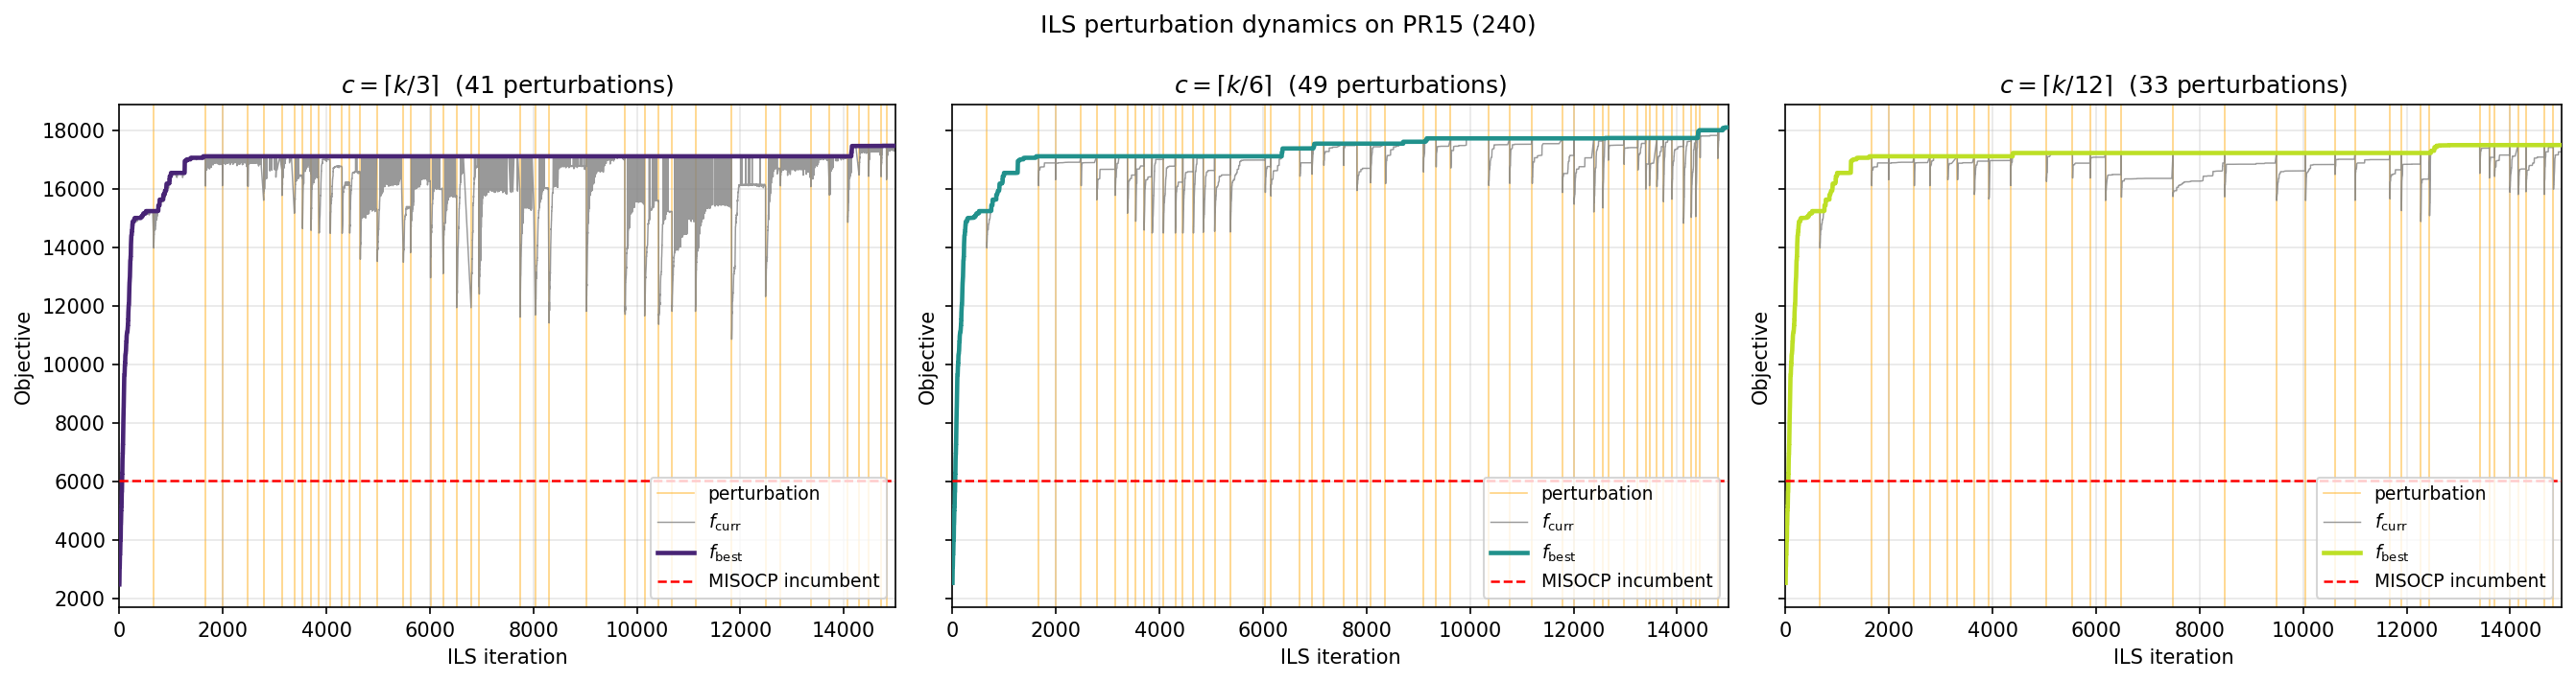
\includegraphics[width=\textwidth]{fig/ils_capdiv.png}
\caption{Perturbation dynamics of the ILS on PR15 (240), one run from R4 per cap divisor $D$, $c = \lceil k/D \rceil$. Grey, the current objective; colored, the best-seen objective; orange lines, the shake steps; dashed, the MISOCP incumbent. Each panel shows the first $15\,000$ iterations, so its shake count is the count within that window and not the count of the whole run reported in Table~\ref{tab:theta}.}
\label{fig:ils-capdiv}
\end{figure}

\subsection{Matheuristic vs.\ exact solver}\label{subsec:matheuristic-vs-exact}

% TEXT REMOVED (September 2026): to be rewritten after the rerun campaign on the expanded benchmark.
% Tables and figures below keep the old results. Plan: UAV-Routing/experiments/RERUN_PLAN.md

% ILS columns refreshed on 2026-09-26 from paper_runs/results/final.csv,
% the single-start runs at the base of Section 4 with maxIter = 13000.
% The MISOCP columns and the Greedy (R4) column are unchanged.

\begin{table}[H]
\centering\footnotesize
\setlength{\tabcolsep}{4pt}
\caption{Greedy (R4) vs.\ single-start matheuristic vs.\ MISOCP at $\eta = 1$, the design of Section~\ref{sec:heuristic} with $c = \lceil k/3 \rceil$. The matheuristic is not capped by the clock and ends after $\mathit{maxIter} = 13\,000$ iterations without an improvement. $t_{\mathrm{best}}$ is the wall-clock time at which the ILS reaches its best solution and Run is the time the whole run takes, the MISOCP gap is from Table~\ref{tab:scalability} (bold marks gap $\le 0.5\%$), and $\Delta = (f^{\star} - f_{\mathrm{best}}^{\mathrm{ILS}})/f^{\star}$ is negative when the ILS beats the MISOCP incumbent.}\label{tab:matheuristic-vs-exact}
\begin{tabular}{l r rrr r r c r}
\toprule
& \multicolumn{1}{c}{Greedy (R4)} & \multicolumn{3}{c}{Single-start ILS ($\mathit{maxIter} = 13\,000$)} & \multicolumn{3}{c}{Exact MISOCP} & \\
\cmidrule(lr){2-2}\cmidrule(lr){3-5}\cmidrule(lr){6-8}
Instance & $f(R_4)$ & $f_{\mathrm{best}}^{\mathrm{ILS}}$ & $t_{\mathrm{best}}$ (s) & Run (s) & $f^{\star}$ & time (s) & gap (\%) & $\Delta$ (\%) \\
\midrule
R101 (50)       & 4\,643.08 & 11\,902.02 & 1 & 12 & \textbf{11\,921.13} & \textbf{7.7} & \textbf{0.00} & $+0.16$ \\
R101 (100)      & 8\,830.33 & 22\,884.32 & 1 & 21 & \textbf{22\,886.91} & \textbf{40.9} & \textbf{0.00} & $+0.01$ \\
R1\_2\_1 (200)  & 5\,758.63 & 16\,586.21 & 26 & 77 & \textbf{16\,954.02} & \textbf{99.6} & \textbf{0.00} & $+2.17$ \\
C101 (50)       & 2\,432.97 & 8\,591.92 & 39 & 240 & 8\,594.11 & 3\,600.0 & 2.61 & $+0.03$ \\
C101 (100)      & 3\,776.53 & 11\,153.74 & 188 & 281 & 11\,328.36 & 3\,600.1 & 32.19 & $+1.54$ \\
C1\_2\_1 (200)  & 2\,583.30 & 11\,083.27 & 39 & 187 & 10\,747.43 & 3\,600.4 & 87.46 & $\mathbf{-3.12}$ \\
RC1\_2\_1 (200) & 4\,198.18 & 17\,669.96 & 64 & 194 & 16\,746.34 & 3\,600.2 & 209.93 & $\mathbf{-5.52}$ \\
R102 (100)      & 13\,854.06 & 30\,443.78 & 62 & 135 & 27\,941.61 & 3\,600.1 & 108.51 & $\mathbf{-8.95}$ \\
R104 (100)      & 15\,524.42 & 38\,060.94 & 169 & 240 & 25\,377.52 & 3\,600.1 & 271.42 & $\mathbf{-49.98}$ \\
C104 (100)      & 9\,670.98 & 18\,233.89 & 379 & 587 & 16\,468.21 & 3\,600.2 & 32.01 & $\mathbf{-10.72}$ \\
RC104 (100)     & 19\,444.49 & 35\,809.19 & 46 & 156 & 27\,439.42 & 3\,600.1 & 289.22 & $\mathbf{-30.50}$ \\
PR11 (48)       & 1\,858.09 & 6\,519.29 & 133 & 227 & 5\,401.01 & 3\,600.0 & 78.53 & $\mathbf{-20.71}$ \\
PR15 (240)      & 2\,471.30 & 18\,221.45 & 579 & 982 & 6\,005.65 & 3\,600.8 & 713.79 & $\mathbf{-203.41}$ \\
PR10 (288)      & 3\,113.48 & 15\,958.48 & 115 & 354 & 5\,377.05 & 3\,600.9 & 984.58 & $\mathbf{-196.79}$ \\
\bottomrule
\end{tabular}
\end{table}

\begin{table}[H]
\centering\footnotesize
\setlength{\tabcolsep}{5pt}
\caption{Value of speed optimization. Protocol of Table~\ref{tab:matheuristic-vs-exact} with the speed fixed at $v_{mr}$ (loitering allowed) or free in $[v_{\min}, v_{\max}]$; Tour counts visited targets.}\label{tab:fixed-speed}
\begin{tabular}{l rr rr r}
\toprule
& \multicolumn{2}{c}{Fixed speed ($v = v_{mr}$)} & \multicolumn{2}{c}{Variable speed} & \\
\cmidrule(lr){2-3}\cmidrule(lr){4-5}
Instance & Obj & Tour & Obj & Tour & Gain (\%) \\
\midrule
R101 (50)       & & & & & \\
R101 (100)      & & & & & \\
R1\_2\_1 (200)  & & & & & \\
C101 (50)       & & & & & \\
C101 (100)      & & & & & \\
C1\_2\_1 (200)  & & & & & \\
RC1\_2\_1 (200) & & & & & \\
R102 (100)      & & & & & \\
R104 (100)      & & & & & \\
C104 (100)      & & & & & \\
RC104 (100)     & & & & & \\
PR11 (48)       & & & & & \\
PR15 (240)      & & & & & \\
PR10 (288)      & & & & & \\
\bottomrule
\end{tabular}
\end{table}

\begin{figure}[H]
\centering
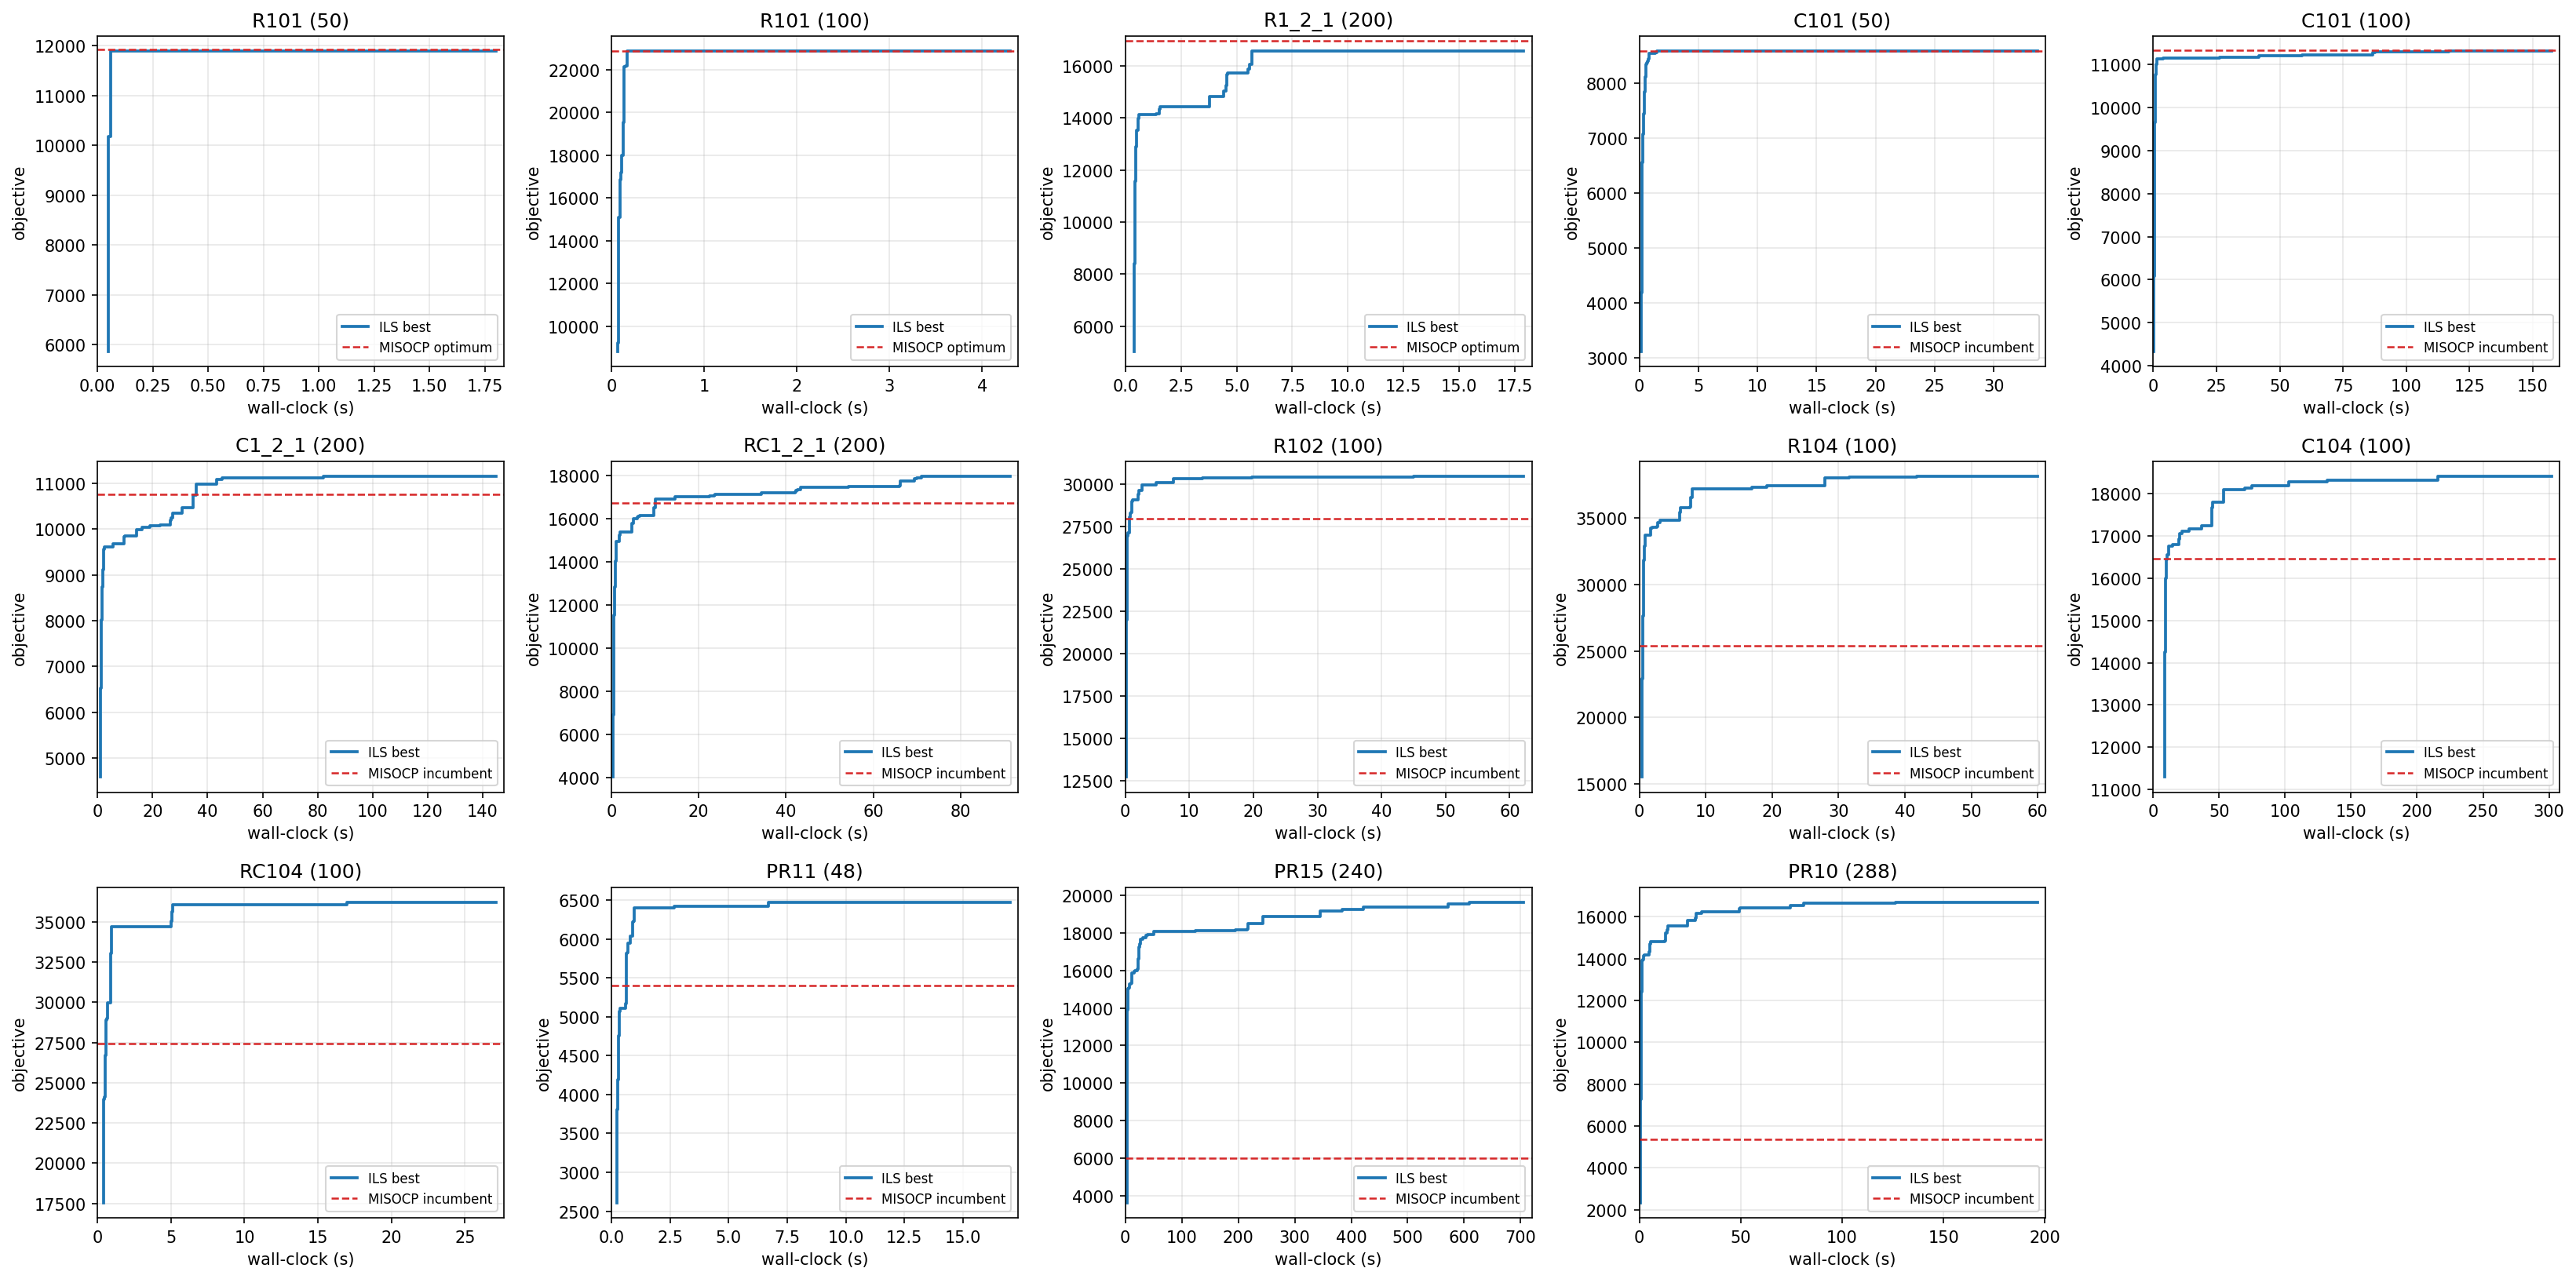
\includegraphics[width=160mm]{fig/meta_convergence_timematched.png}
\caption{ILS convergence under the protocol of Table~\ref{tab:matheuristic-vs-exact}: best-seen objective against wall-clock time, one panel per instance. Each panel ends where its run ends, since the iteration limit of Section~\ref{subsec:ils} stops each instance at its own time rather than at a common budget. The dashed line is the MISOCP value at the $3\,600$\,s cap, a proven optimum or the incumbent.}
\label{fig:ils-convergence}
\end{figure}


% ============================================================
\subsection{Value of loitering for the matheuristic}\label{subsec:coverage}

% TEXT PENDING: the count of scheduled targets is not a proxy for the objective
% under time-dependent rewards. A target squeezed into a route delays every later
% arrival, so on instances whose rewards move quickly within the window the best
% route may visit fewer targets than a worse one. The measured contrast runs the
% other way from the naive expectation: fixing the speed does not sharpen the
% conflict, it removes it, because with no speed to trade the route can only win
% by covering more. State that, and note that both blocks are filled.

\begin{table}[H]
\centering\small
\setlength{\tabcolsep}{5pt}
\caption{Value of loitering for the matheuristic. Protocol of Table~\ref{tab:matheuristic-vs-exact} with the flight length pinned to the straight-line distance, $L_{ij} = d_{ij}$, or free to exceed it; the speed varies in $[v_{\min}, v_{\max}]$ in both settings. $k$ counts scheduled targets and Tour is the flown length. Loitering lets the drone delay an arrival by flying further rather than by flying slower, which is the only way to reach a late-opening window once the speed is already at $v_{\min}$, and it costs energy. The rows to read are those where the loitering route schedules fewer targets, or covers a shorter tour, and still collects more information: there the extra flight bought timing rather than coverage.}\label{tab:coverage}
\begin{tabular}{l rrr rrr r}
\toprule
& \multicolumn{3}{c}{No loitering ($L_{ij} = d_{ij}$)} & \multicolumn{3}{c}{Loitering allowed} & \\
\cmidrule(lr){2-4}\cmidrule(lr){5-7}
Instance & Obj & $k$ & Tour (km) & Obj & $k$ & Tour (km) & Gain (\%) \\
\midrule
R101 (50)       &  &  &  &  &  &  &  \\
R101 (100)      &  &  &  &  &  &  &  \\
R1\_2\_1 (200)  &  &  &  &  &  &  &  \\
\midrule
C101 (50)       &  &  &  &  &  &  &  \\
C101 (100)      &  &  &  &  &  &  &  \\
C1\_2\_1 (200)  &  &  &  &  &  &  &  \\
\midrule
RC1\_2\_1 (200) &  &  &  &  &  &  &  \\
\midrule
R102 (100)      &  &  &  &  &  &  &  \\
R104 (100)      &  &  &  &  &  &  &  \\
C104 (100)      &  &  &  &  &  &  &  \\
RC104 (100)     &  &  &  &  &  &  &  \\
\midrule
PR11 (48)       &  &  &  &  &  &  &  \\
PR15 (240)      &  &  &  &  &  &  &  \\
PR10 (288)      &  &  &  &  &  &  &  \\
\bottomrule
\end{tabular}
\end{table}

\section{Conclusion} \label{sec:conc}

% TEXT REMOVED (2026-09-24): the conclusion quoted matheuristic results
% throughout, and every ILS number predates the evaluated-route store fix.
% To be rewritten after the rerun campaign. The removed text, including the
% open-directions list, is kept in the session scratchpad as
% conclusion_removed_2026_09_24.tex.

\bibliographystyle{amsplain}
\bibliography{ref}

\end{document}


